\documentclass[continuous]{grattan}\usepackage[]{graphicx}\usepackage[]{color}
%% maxwidth is the original width if it is less than linewidth
%% otherwise use linewidth (to make sure the graphics do not exceed the margin)
\makeatletter
\def\maxwidth{ %
  \ifdim\Gin@nat@width>\linewidth
    \linewidth
  \else
    \Gin@nat@width
  \fi
}
\makeatother

\definecolor{fgcolor}{rgb}{0.345, 0.345, 0.345}
\newcommand{\hlnum}[1]{\textcolor[rgb]{0.686,0.059,0.569}{#1}}%
\newcommand{\hlstr}[1]{\textcolor[rgb]{0.192,0.494,0.8}{#1}}%
\newcommand{\hlcom}[1]{\textcolor[rgb]{0.678,0.584,0.686}{\textit{#1}}}%
\newcommand{\hlopt}[1]{\textcolor[rgb]{0,0,0}{#1}}%
\newcommand{\hlstd}[1]{\textcolor[rgb]{0.345,0.345,0.345}{#1}}%
\newcommand{\hlkwa}[1]{\textcolor[rgb]{0.161,0.373,0.58}{\textbf{#1}}}%
\newcommand{\hlkwb}[1]{\textcolor[rgb]{0.69,0.353,0.396}{#1}}%
\newcommand{\hlkwc}[1]{\textcolor[rgb]{0.333,0.667,0.333}{#1}}%
\newcommand{\hlkwd}[1]{\textcolor[rgb]{0.737,0.353,0.396}{\textbf{#1}}}%
\let\hlipl\hlkwb

\usepackage{framed}
\makeatletter
\newenvironment{kframe}{%
 \def\at@end@of@kframe{}%
 \ifinner\ifhmode%
  \def\at@end@of@kframe{\end{minipage}}%
  \begin{minipage}{\columnwidth}%
 \fi\fi%
 \def\FrameCommand##1{\hskip\@totalleftmargin \hskip-\fboxsep
 \colorbox{shadecolor}{##1}\hskip-\fboxsep
     % There is no \\@totalrightmargin, so:
     \hskip-\linewidth \hskip-\@totalleftmargin \hskip\columnwidth}%
 \MakeFramed {\advance\hsize-\width
   \@totalleftmargin\z@ \linewidth\hsize
   \@setminipage}}%
 {\par\unskip\endMakeFramed%
 \at@end@of@kframe}
\makeatother

\definecolor{shadecolor}{rgb}{.97, .97, .97}
\definecolor{messagecolor}{rgb}{0, 0, 0}
\definecolor{warningcolor}{rgb}{1, 0, 1}
\definecolor{errorcolor}{rgb}{1, 0, 0}
\newenvironment{knitrout}{}{} % an empty environment to be redefined in TeX

\usepackage{alltt}
%\input{preamble}
\title{A better super system: Assessing the 2016 tax reforms}
\author{John Daley, Brendan Coates and William Young}

\hypersetup{pdfauthor = {John Daley and Brendan Coates and William Young and Hugh Parsonage},
pdftitle = {A better super system: assessing the 2016 tax reforms, Version 1.4.0}
}

%\GrattanWorkingPaperNumber{2016-1.4}
%\GrattanReportNumber{2016-1.4}

\addbibresource{AP-bib/bibliography.bib}
\addbibresource{bibliographyRpackages.bib}



% Following is just for safety. Prevents inadvertent entry
% into mathmode -- e.g. 'With $1000, you can buy 1000 $1 things.' 
% \catcode`\$=12















% I should have just used `+`(...) 






\acknowledgements{%
This working paper was written by John Daley, Brendan Coates and William Young.
Hugh Parsonage provided extensive research assistance and made substantial contributions to the paper.

We would like to thank numerous people from the public policy community and Grattan Institute's Public Policy Committee for their helpful comments.

The opinions in this report are those of the authors and do not necessarily represent the views of Grattan Institute's founding members, affiliates, individual board members, reference group members or reviewers.
Any remaining errors or omissions are the responsibility of the authors.

Grattan Institute is an independent think-tank focused on Australian public policy.
Our work is independent, practical and rigorous.
We aim to improve policy outcomes by engaging with both decision-makers and the community.
For further information on the Institute's programs, or to join our mailing list, please go to: \textcolor{blue}{\url{http://www.grattan.edu.au/}}

{\footnotesize
This working paper may be cited as Daley, J., Coates, B., Young, W., and Parsonage, H., \emph{\mytitle}, 2016, Grattan Institute

978-1-925015-90-4

All material published or otherwise created by Grattan Institute is licensed under a Creative Commons Attribution-NonCommercial-ShareAlike 3.0 Unported License\par
}
}
\IfFileExists{upquote.sty}{\usepackage{upquote}}{}
\begin{document}

% cosmetic
\addtolength{\columnsep}{3.5mm}
\begin{overview}[-2.2\baselineskip]
Winding back superannuation tax breaks will be an acid test of our political system. 
Not because our major political parties are at loggerheads, but because they largely agree on both ends and means. 
If we cannot get reform in this situation, then there is little hope for either budget repair or wider economic reform.

Better targeting of superannuation tax breaks should be one of the first items of business in the new Federal Parliament.
The government proposes to legislate that the aim of the \$2 trillion superannuation system is to encourage savings to supplement or substitute for the Age Pension.
Tax breaks should only be available when they serve this policy aim.
Yet as our \citeyear{DaleyCoatesWoodEtAl2015Super} \citetitle{DaleyCoatesWoodEtAl2015Super} report shows, current super tax breaks go well beyond this purpose and their costs are unsustainable.

This paper analyses the impact of proposed changes to super tax breaks announced in the May Budget by the Coalition Government, and the \ALP{}’s subsequent policy response. 
They largely agree on a new 15 per cent tax on super earnings in retirement for those with super account balances of more than \$1.6~million; a lower annual cap of \$25,000 on pre-tax contributions; a lower income threshold of \$250,000 at which tax on super contributions will rise from 15 to 30~per cent; a \$500,000 lifetime cap on post-tax contributions; taxing earnings while in transition to retirement; and removing tax breaks on inheritance. 

These would be big steps towards aligning super tax breaks more closely with their purpose. 
They would trim the generous super tax breaks enjoyed by the top 20 per cent of income earners – people wealthy enough to be comfortable in retirement and unlikely to qualify for the Age Pension. 

Claims that the Budget changes will affect many low- and middle-income earners are wrong.
The changes will affect about 4 per cent of superannuants, nearly all of them high-income earners who are unlikely to access the Age Pension. 
Nor are the proposed changes retrospective.
Many reforms affect investments made in the past, and no-one suggests they are retrospective.
Rather, the changes will affect taxes paid on future super earnings, and entitlements to make future contributions to super. 

The major parties disagree about relatively little in this reform debate. 
The \ALP{} would not count post-tax contributions between 2007 and the present. 
On the other hand it would adopt a number of other policies that would contribute even more to budget repair. 
Any combination of the packages on offer would improve the current system overall. 

The changes are electorally popular. 
Electorates more likely to be adversely affected by the super changes – that is, those with more old and wealthy voters – tended to swing less to the \ALP{} at the last election than other electorates. 
A survey before the election showed that the proposals had more support amongst those most likely to be adversely affected.

The proposed changes to super tax are built on principle, supported by the electorate, and largely supported by all three main political parties. 
If common ground cannot be found in this situation, then our system of government is irredeemably flawed. 

Even after the reforms, super tax breaks will still mostly flow to high-income earners who do not need them. 
The budgetary costs of super tax breaks will remain unsustainable in the long term.
Further changes to super tax breaks will be needed in future.
\end{overview}
\addtolength{\columnsep}{-3.6mm}

% \begin{table*}
\onecolumn
\thispagestyle{empty}
% Position table at center
\catcode`\$=3







\begin{tikzpicture}[remember picture, overlay]






% Center hoirzontally
\node[inner sep = 0pt] (SummaryTable) at (current page.center) {%
\input{tex/table1}
};
\node[above = 3pt of SummaryTable, text width = \paperwidth, inner sep = 0pt] (caption)
  {\captionsetup{margin = {0.0625\paperwidth,0cm}}
   \captionof{table}[Summary of positions table]{Government proposed reforms to superannuation tax breaks, ALP responses, and Grattan recommendations\label{tbl:Summary-table}}
};
%                                               0.935\paperwidth = magical to align >|Source with left of table 
\node[below = 3pt of SummaryTable, text width = 0.87\paperwidth, inner sep = 0pt] (belowcaption)
  {\footnotesize\textit{Source:~Grattan analysis of \textcites{BudgetPapers201617}{ATO2016SampleFile1314}{ALP-2016-Making-super-fairer}.}
};
\end{tikzpicture}
% \catcode`\$=12  % for tikz
% \end{table*}
\twocolumn
\AtBeginEnvironment{tabular}{\small}  % for subsequent tables



\contentspage

\clearpage
\listoffigures
\clearpage

\chapter{Introduction}\label{chap:intro}
\section{Aims for the superannuation system}\label{aims-for-the-superannuation-system}
Despite accumulating more than \$2 trillion in assets under management, our superannuation system has never had legislated aims.%
\footcite{APRA2016-Annual-Superannuation-Bulletin-Jun2015} %
This is changing.

The \citeyear{FinancialSystemsInquiry2014} \citetitle{FinancialSystemsInquiry2014} recommended that superannuation should provide `income in retirement to substitute or supplement the Age Pension.'\footcites{FinancialSystemsInquiry2014}{DaleyCoatesWoodEtAl2015Super} %
The Coalition endorsed this view in the May 2016 Budget.%
\footcites[][5]{Budget-2016-17-Tax-Super}{Morrison-2016-A-more-sustainable-superannuation-system} %
The \ALP{} also backed legislating an objective for superannuation -- although it has not yet committed to the objective proposed by the Financial System Inquiry.%
\footnote{\textcite{Bowen-Objective-Super-2016}. In a speech in \citeyear{Bowen-June-2015-speech-to-committee-for-sustainable-retirement-incomes}, the Shadow Treasurer Chris Bowen proposed `our superannuation system should ensure that as many Australians as possible have access to the resources for a dignified retirement without recourse to the full age pension' 
(\textcite{Bowen-June-2015-speech-to-committee-for-sustainable-retirement-incomes}).}

As our recent \citetitle{DaleyCoatesWoodEtAl2015Super} report shows, if the objective of super is to provide retirement income to substitute for or supplement the Age Pension, then the system should avoid supporting those whose wealth makes them unlikely to receive even a part Age Pension. %
This objective also implies that superannuation should not support savings at a high cost to the budget if it only reduces Age Pension liabilities a little. %
The benefits of higher retirement incomes must be balanced against the costs of achieving them.\footnote{See \textcite[][16]{DaleyCoatesWoodEtAl2015Super}.} 

Yet current superannuation tax breaks often go well beyond this purpose and their costs are unsustainable.
The tax breaks reduce income tax collections by more than \$25~billion a year.\footnote{As noted in \citetitle{DaleyCoatesWoodEtAl2015Super}, this estimate accounts for behavioral change, where people would put less money into superannuation and more into other vehicles where they pay less tax than their marginal rate of income tax. See \textcite{DaleyWoodCoates2015} and \textcite[][23--24]{DaleyCoatesWoodEtAl2015Super}. %
The value of superannuation tax breaks is calculated against a
comprehensive income tax benchmark. While some commentators argue that an
expenditure tax approach is a desirable structural feature of the tax system,
arguments about the best policy for taxing savings should not be confused with
questions about how to measure their cost. The income tax benchmark remains
the best measure of how much tax breaks cost. Absent superannuation, savings
would be taxed at rates of personal income tax. See: \textcite[][Box~1]{DaleyCoatesWoodEtAl2015Super}.
} 
More than half the benefits flow to the wealthiest 20 per cent of households who already have enough resources to fund their own retirement, and whose savings choices aren't affected much by tax rates. %
The current system is expensive and unfair. 
Reforms, such as those proposed by the major parties are sorely needed.

\section{Contributing to budget repair, and restoring the intergenerational bargain}\label{sec:contributing-to-budget-repair-and-restoring-the-intergenerational-bargain}

Apart from being needed to align super with its policy rationale, \mbox{reforms} are also needed to contribute to budget repair, and to restore the intergenerational bargain.

The Commonwealth budget has a serious structural deficit.
Actual deficits have been around 2 to 3 per cent of GDP for eight years.%
\footcite[][4]{DaleyWood2015FiscalChallenges} %
The Government is yet to respond to the scale of this budget challenge.
In office, both major political parties have hoped that bracket creep and favourable economic conditions would deliver a surplus.
Yet over seven years, outcomes have consistently been worse than these projections.%
\footcite{DaleyWood-2016-theConvo-3-critical-tests-for-budget-2016} %
Age-based spending and tax breaks are major contributors to structural deficits. 

Net government transfers per household are calculated as the total of health, education and welfare spending less income and consumption taxes.
Between 2004 and 2010, average net government transfers to households over the age of 65 increased in real terms from  \$23,000 to \$32,000 per household over the age of~65.%{
\footcite[][22]{DaleyWoodWeidmannEtAl2014} %
The increase in net transfers to older households has worsened Australian government budgets by \$22~billion a year.\footcite[][22]{DaleyWoodWeidmannEtAl2014}

For more than a decade, superannuation tax breaks have been absurdly generous to older people on high incomes.
They are one of the major reasons why households over the age of 65 (unlike households aged between 25 and 64) are paying less income tax in real terms today than they did 20 years ago, even though their workforce participation rates and real wages have jumped (\Vref{fig:change-in-taxes-per-hhold-WOG}).%
\footcite[][27]{DaleyWoodWeidmannEtAl2014} 

\begin{figure}
\captionwithunits{Older households are paying less income tax because of the super tax breaks\label{fig:change-in-taxes-per-hhold-WOG}}%
{Real change in taxes per household, 1988-89 to 2009-10, (2010 dollars)}
\begin{knitrout}
\definecolor{shadecolor}{rgb}{0.969, 0.969, 0.969}\color{fgcolor}
\includegraphics[width=4.47222in,height=2.94759954545455in]{atlas/change-in-taxes-per-hhold-WOG-noQC-1} 

\end{knitrout}
\source{\textcite[][Figure~3.6]{DaleyWoodWeidmannEtAl2014}.}
\end{figure}

In particular the decision by the former Coalition Government to abolish taxes on superannuation withdrawals for those aged over 60 years in 2007 -- without introducing taxes on super fund earnings in retirement -- dramatically reduced the income tax bills of older Australians.\footnote{\label{footnote:Simple-super-reforms}Tax-free super withdrawals for over~60s were introduced by the former Howard Government as part of the \textit{Simpler Super} reforms. 
Prior to that, super income streams were taxed at marginal rates of personal income tax less a 15~per cent rebate, whereas lump sums were taxed at different rates depending on whether they exceeded reasonable benefit limits (\textcite{Treasury2008RetirementIncomeConsultPaper}). 
Superannuation schemes where contributions are not taxed, such as public-service defined benefit pensions, still have taxes applied to withdrawals.} 

Changes to superannuation tax arrangements in 2008 materially increased the number of income “taxed nots”\footnote{%
This expression was introduced in \textcite{Morrison-2016-have-havenots-speech}. 
We interpret it here as the number of people paying income tax. 
Of course, virtually all households pay indirect taxes, and about half of all households receive more in benefits and services than they pay in taxes, because total government spending on welfare and services is similar to income and indirect taxes paid. 
\textcite{Jericho-theGuardian-on-Morrisons-have-havenots-speech}.%
}  aged over 65 (\Vref{fig:prop-population-paying-personal-income-tax-by-age-1999}). %
The introduction of tax-free super benefits provided an enormous windfall to high-income earners that had already amassed large super account balances that were no longer liable for taxes on either fund earnings or benefits withdrawn.\footnote{%
Prior to 2007, the amount of concessionally taxed benefits superannuation benefits that people were allowed to receive over their lifetime was limited by reasonable benefit limits. 
The system was complex to administer and affected few taxpayers. 
However, it ensured that those with very large super balances paid additional taxes when they made large super withdrawals. 
Recent \ASFA{} estimates suggested that 475~people with super account balances greater than \$10~million are drawing tax-free income streams at an average of \$1.5~million annually. See \textcites[][10]{Parl-Lib-2005-Super-ready-reckoner-multiple-rules-for-200506}[][106]{Super-Select-Committee-2002-Super-standards-living-retirement}[][4]{Clare2015-Super-high-account-bals}.}

Making a transition to a fairer set of policies requires careful thought. 
Younger generations, on the wrong side of the drawbridge after the policies change, lose out when they pay for benefits for older generations that they do not receive themselves. 
Exempting older households from the costs of policy changes – by grandfathering existing benefits and tax breaks, for example – simply magnifies the costs shifted onto younger generations.

\begin{figure}





% \captionsetup{oneside, margin = {0cm,-0.5cm}}
% \captionwithunits{In stark contrast with the working population, the number of tax-paying individuals over 65 has not reflected population growth\label{fig:prop-population-paying-personal-income-tax-by-age-1999-to-2013}}%
% {Population and population paying tax, by age group, 1999-00 = 100}%
\captionsetup{oneside, margin = {0cm,-0.5cm}}
\captionwithunits{Older Australians account for a large share of the “taxed nots”\label{fig:prop-population-paying-personal-income-tax-by-age-1999}}
{Proportion of population paying personal income tax by age}
\begin{knitrout}
\definecolor{shadecolor}{rgb}{0.969, 0.969, 0.969}\color{fgcolor}
\includegraphics[width=4.8299976in,height=2.94759954545455in]{atlas/prop-population-paying-personal-income-tax-by-age-1999-to-2013-1} 

\end{knitrout}


\noteswithsource{Individuals paying income tax are those as identified by the \ATO{} at the time the \ATO{} statistics for that tax year were released. %
Late taxpayers are probably about another 5~per cent of the
population, but the bias is likely to be constant across the time series. Population
data is for March quarter of each tax year. \SATO{} and the Pensioner Tax
Offset were amalgamated into the Seniors and Pensioners Tax Offset
(\SAPTO{}) in 2012\nobreakdash-13.}%
{Grattan analysis of \textcites{ATO19992015}{ABS-2016-Resident-population-by-quarter}.}
\end{figure}



\section{Political recognition of the need for reform}\label{political-recognition-of-the-need-for-reform}

In the recent Federal election campaign, both major parties proposed rolling back superannuation tax breaks.
The Turnbull Government announced a super reform package in the May 2016 Budget.%
\footcite{Morrison-2016-A-more-sustainable-superannuation-system} The \ALP{} had announced its own reforms to super tax breaks in late 2015,\footcite{ALP2015FairerSuper} and committed to reviewing the Coalition's proposed changes after the Federal election.%
\footcite{Chalmers-Further-consultation-on-Govt-super} %
In August 2016 the \ALP{} released a revised super package, which would save \$1.7~billion more over four years than the government’s plan.\footcite{Bowen-2016-Labors-plan-for-super-not-retrospective}

There is little evidence for the claim that the Government's proposals reduced support for the Coalition in the 2016 Commonwealth election.\footcite{ABC-Lib-campaign-failed-to-resonate-Abetz-sez} %
The ten electorates most affected by the Coalition’s proposed changes swung less to the \ALP{} than the national average – indeed some swung towards the Coalition.\footnote{\textcite{Mather-Evidence-lacking-of-voter-backlash-super-changes}. \textcite{Pollbludger-Election2016-post-mortem} shows that electorates with a greater proportion of older people with higher median incomes – those most affected by the Coalition’s super changes – swung less against the Coalition Government than the national average after accounting for other factors.} %
Polling suggests that support for the changes is highest amongst older people on high incomes\footnote{Those most likely to approve of the \$1.6~million cap on tax-free super earnings in retirement were Liberal/National voters (57 per cent), full-time workers (53 per cent), those earning \$1500-2000 a week (57 per cent) and those making after-tax super contributions (60 per cent). \textcite{EssentialMedia-June2016}.}  – perhaps because they understand that the current system is unsustainable. 
In the face of these facts, some arguments against the superannuation proposals seem to amount to a claim that they should not proceed simply because Coalition party donors oppose them,\footcite{theOz-Morrison-super-policy-alienated-Libs} %   
which is not usually considered a relevant consideration for policy decisions. 

Reforms to super tax breaks represent a rare opportunity to make much-needed progress on budget repair, while better aligning super tax breaks with their policy purpose. 
Both major parties agree on many measures. 
The risk is that these disagreements will derail reform. 
Good politics is always the art of compromise. 

\section{This paper's analysis of 2016 Budget reforms and opposition proposals}\label{this-papers-analysis-of-2016-budget-reforms}

The remainder of this paper analyses the impact of proposals made by the major parties to wind back super tax breaks. 
It considers who would be affected and by how much.
More importantly, it examines whether the proposals would better align super tax breaks with the newly articulated purpose of super.

\Cref{chap:proposed-reforms-to-contributions-tax-breaks} evaluates the proposed changes to \textbf{contribution tax breaks} announced in the 2016 Budget.
\Cref{chap:proposed-reforms-to-earnings-tax-breaks} evaluates the proposed changes to \textbf{earnings tax breaks}.

\Cref{chap:proposed-reforms-to-total-super-contributions} considers changes to \textbf{how much in total people can contribute to superannuation}, including from their post-tax income, and the rules governing when they can make contributions.
\Cref{chap:how-many-people-will-be-adversely-affected-by-the-super-changes} considers \textbf{how many people in total will be adversely affected} by the proposed changes.

\Cref{chap:contr-to-budget-repair} analyses their budgetary impact. 
\Cref{chap:future-changes} asks \textbf{whether the proposed changes go far enough} to align super with its new purpose. 











\chapter{{Proposed reforms to contributions tax breaks}}\label{chap:proposed-reforms-to-contributions-tax-breaks}
\section{Targeting pre-tax contribution tax breaks where they are needed}\label{sec:targeting-pre-tax-contribution-tax-breaks-where-they-are-needed}
People can contribute to superannuation from their pre-tax income. 
These “concessional” contributions are taxed at just 15 per cent, rather than the person’s marginal income tax rate.

\subsubsection{Tightening access to contributions tax breaks}\label{subsubsec:tightening-access-to-contributions-tax-breaks}
The Government’s super package will reduce how much people can contribute to superannuation from their pre-tax income.  
The limit will be reduced from \$30,000 (or \$35,000 for over~50s) to \$25,000 a year. 
Furthermore, contributions will be taxed at 30~per cent rather than 15~per cent if a person earns more than \$250,000 – down from the current threshold of \$300,000.\footcite{ATO2016Div293-Info-for-individuals} %
Treasury expects the changes will bring in an extra \$1.2~billion a year by 2019-20.\footcite[][28]{BudgetPapers201617} 

These changes will better align superannuation tax breaks with their policy purpose by reducing tax breaks for those who don’t need them as a substitute for the Age Pension. 
The changes will affect about 520,000 people in 2017-18 -- overwhelmingly high-income earners who are unlikely to access the Age Pension in retirement.%
\footnote{Grattan analysis of \textcite{ATO2016SampleFile1314}.} 
Almost three-quarters of the people affected are in the top fifth of income earners (\Vref{fig:Total-pre-tax-contributions}).

\begin{figureTop}
\Caption{Trimming pre-tax contribution tax breaks will mainly affect the wealthiest Australians}%
{Total superannuation contributions tax breaks, 2017-18 projections}%
{fig:Total-pre-tax-contributions}


\begin{knitrout}
\definecolor{shadecolor}{rgb}{0.969, 0.969, 0.969}\color{fgcolor}
\includegraphics[width=4.695831in,height=3.2423595in]{atlas/total-superannuation-tax-breaks-by-taxable-income-decile-201718-1} 

\end{knitrout}
\noteswithsource{The value of tax break is calculated against a comprehensive income tax
benchmark. Does not include the impact of the Low Income Superannuation Tax Offset.}%
{Grattan analysis of \textcite{ATO2016SampleFile1314}.}
\par\null
\vfill
\null
\end{figureTop}


The Government will also remove the anti-detriment provision that effectively refunds the taxes paid on super contributions if a member dies and the beneficiary is a dependant. 
There is no justification for boosting the value of inherited super balances -- super is not a taxpayer-funded inheritance scheme. 
Treasury expects this change will raise \$245~million a year by 2019-20.

The \ALP{} supports the Government’s moves to tighten access to contributions tax breaks, accepting the government’s moves to tighten the annual cap on pre-tax super contributions to \$25,000 a year and the removal of anti-detriment provisions.\footcites{Bowen-2016-Labors-plan-for-super-not-retrospective}{DaleyCoates-2016-theConvo-A-super-test-for-Aus-pol-system} %  

Labor also proposes that the new income threshold for the 30~per cent tax rate on pre-tax super contributions be lowered further to \$200,000, which would save an additional \$500~million a year by 2019\nobreakdash-20, compared to the Government’s plan. 
In practice this more or less aligns with the top marginal income tax rate of \$180,000 because the income threshold for pre-tax super contributions includes both income and super contributions. 
It would mean that overall the system would broadly provide all taxpayers with a discount from their marginal income tax rate for superannuation contributions of between 15 and 22 per cent. 

Lowering the income threshold even further for the 30~per cent tax rate to \$180,000, thereby aligning it with the top marginal rate of personal income tax, would save the budget a further \$350~million a year.\footnote{Grattan analysis of \textcite{ATO2016SampleFile1314}.} 

\subsubsection{Boosting contributions tax breaks for low-income workers}\label{subsec:boosting-contributions-tax-breaks-for-low-income-workers}

The Government will also boost super tax breaks for low-income earners by retaining the Low Income Superannuation Contribution (\LISC{}), now renamed the Low Income Superannuation Tax Offset~(\LISTO{}) and paid through the tax system. 
The \LISC{} is due to be abolished in 2017-18. %\enlargethispage*{0.25\baselineskip}\enlargethispage{0.25\baselineskip}







The \LISTO{} removes a tax penalty on some low\nobreakdash-income people, who pay more tax on their super contributions than on their take-home pay. % 
In 2017-18, it will provide \$800~million\footcite[][28]{BudgetPapers201617}  to 3.3~million\footcite[][Fact Sheet No.~06]{Budget-2016-17-Super-fact-sheets} individuals on less than \$37,000 a year. 
%\footnote{Our estimates: texNum(LISTO_stats$Expenditure, dollar = TRUE) to texNum(LISTO_stats$N_pers) taxpayers.}
The \ALP{} also supports this proposal.\footcite{Bowen-2016-Labors-plan-for-super-not-retrospective}

Yet it remains unclear whether the best way to improve retirement incomes for low-income earners is to provide extra super tax breaks such as the \LISTO{}, or additional Age Pension support. 
Of course, this trade-off assumes that money saved by not proceeding with the \LISTO{} is re-directed towards additional Age Pension support. 
While such cross-portfolio budgetary transfers are uncommon, there are precedents, particularly for such a large strategic shift. 

On the one hand, the \LISTO{} is well-targeted to boost the super balances of low-income workers. 
Boosting individuals’ superannuation balances, particularly women's, may improve their economic independence.\footnote{For example, see \textcite[][90--91]{Senate-Ref-Committee-2016-Achieving-econ-security-women-retirement}.} 
The \LISTO{} also compensates low-income earners for being compelled to lock up their savings in superannuation in retirement.\footcite[][17]{DaleyCoatesWoodEtAl2015Super}   

On the other hand, government may be able to deliver more effective and targeted assistance to low-income groups through income support payments rather than through superannuation. 
Boosting the retirement incomes of low-income earners delivered through the tax and superannuation systems are also inherently less well-targeted than increasing income support payments, which take into account the resources of the entire household. 

For example, government makes additional co-contributions when people with low incomes make voluntary post-tax super contributions. 
But it is likely that most who will benefit from these provisions are the partners of high-income earners.%
\footcite[][4]{Grattan-submission-2016-Senate-Inq-econ-security-women-retirement} %
Therefore boosting retirement incomes through superannuation may produce a less progressive tax system overall. 

Further, the \LISTO{} may provide only a limited boost per budgetary dollar to the retirement incomes of low-income earners. %
Low-income earners accumulate less super, and so fees can erode a larger portion of their contributions.\footnote{%
\textcite{Rice-Warner-2012-Super-fees-research} found that super fees for low-balance accounts can be much larger than the industry average. 
Account administration fees are typically charged at a flat rate irrespective of the super account balance, as are default insurance premiums provided by super funds (\textcites{ASIC-2016-Super-fees}{Canstar-2016-Guide-to-understanding-super-fees}). 
\textcite[][8]{Minifie-Savage-Cameron-2014-Super-sting} showed that small increases in fees can have a significant effect on account balances at retirement. 
}   
More evidence is needed to test how much of the \LISTO{} will ultimately benefit low-income retirees, and how much will be eroded in fees.
Super funds could calculate this based on member records, or Treasury could derive it from longitudinal analysis of individual tax records that include both superannuation contributions and balances.



\subsubsection{Expanding access to contributions tax breaks to all workers}\label{expanding-access-to-contributions-tax-breaks-to-all-workers}
Finally, the 2016 Budget proposes to make it easier for people to make voluntary pre-tax contributions directly to their superannuation fund. 
Under the changes, all taxpayers will be able to contribute directly to their super fund and claim a tax deduction on their personal income tax return. 
At present, only people who earn most of their income from non-employment activities (usually people who are self-employed or drawing most of their income from investments) can contribute directly;\footcite{ATO-2016-Claiming-deductions-for-pers-super-contr} %
employees and those with a mixture of part-time work and self-employment can only make pre-tax voluntary contributions if their employer provides a facility for salary sacrifice contributions.

The change improves system flexibility and levels the playing field so that some people do not miss out on super tax breaks simply because of their employment circumstances.
In particular, the bulk of workers denied access to salary sacrifice arrangements are likely to work for small employers earning lower wages.\footcite[][Table~13]{ABS-May-2014-Employee-earnings-and-hours} 

Treasury expects 850,000~workers to use these new arrangements. By 2019-20 they will receive a further \$750~million of super tax breaks a year -- at the expense of the Commonwealth Treasury.\footnote{%
  For the number of people affected, see \textcite[][5]{Budget-2016-17-Super-fact-sheets}; for the revenue figure, see \textcite[][25]{Budget-2016-17-Tax-Super}. The budgetary cost of the new system matures in 2019\nobreakdash-20: until then there are timing effects because tax is paid on extra contributions, but deductions for them are only paid out in the following fiscal year.%
} 

The \ALP{} does not support this proposal.\footcite{Bowen-2016-Labors-plan-for-super-not-retrospective}
It argues that those using the new arrangements are likely to be mainly high-income earners, and providing them with additional support should not be a priority given budgetary constraints. 

But the government’s proposal does promote consistency. 
If pre-tax contributions are allowed at all, there is no reason in principle to lock out people with employers who have less sophisticated payroll systems.
One of the overall reform objectives should be to make superannuation policy more stable by aligning the system with its purpose.


\section{Pre-tax contribution limits are sufficient for those with broken work histories}\label{sec:pre-tax-contribution-limits-are-sufficient-for-broken-work-histories}

Some have suggested that the lower \$25,000 annual cap on pre-tax super contributions will make it harder for those with broken work histories -- particularly women and carers -- to make catch-up super contributions.%
\footcites{SMSF-Assoc-2016-Super-changes-cause-concern}{NATSEM-2016-Impact-of-201617-super-changes-by-gender-age} %
Such concerns are overblown. %
All the evidence shows that very few middle-income earners, and even fewer women, make large catch-up contributions to their super funds.%
\footcite{Grattan-submission-2016-Senate-Inq-econ-security-women-retirement} 

















\begin{figure}%
\Caption{Pre-tax contributions of more than \$25,000 a year will likely be made mainly by high-income men}%
{Projected number of individuals in 2017-18 making pre-tax contributions of more than \$25,000}%
{fig:pre-tax-contributions-25k-by-decile-201718}
\begin{knitrout}
\definecolor{shadecolor}{rgb}{0.969, 0.969, 0.969}\color{fgcolor}
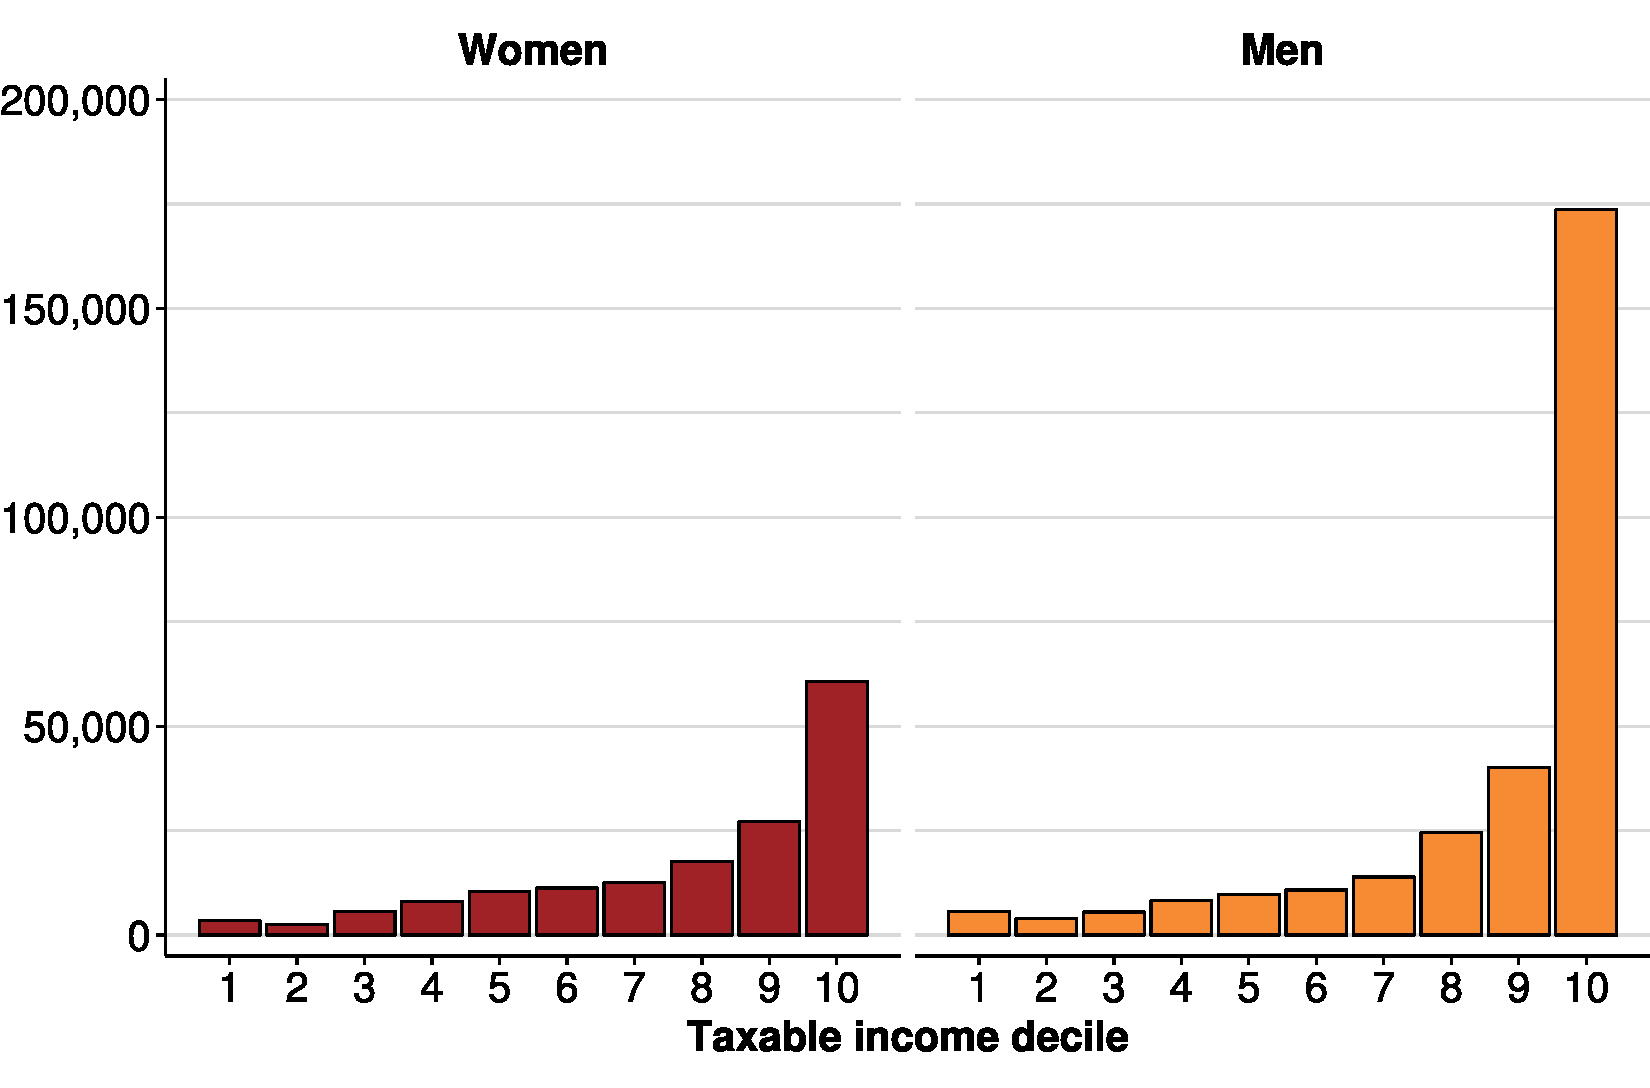
\includegraphics[width=4.47222in,height=2.94759954545455in]{atlas/n-individuals-contr-over-25k-by-decile-201718-1} 

\end{knitrout}
\noteswithsource{Pre-tax super contributions made by individuals in the ATO 2 per cent
sample file for 2013-14 are adjusted to reflect total pre-tax contributions reported
in ATO Taxation Statistics for superannuation funds, such as by estimating
Super Guarantee contributions for taxpayers with salary income but who report
no pre-tax contributions from their employer and accounting for people who do
not lodge their tax return on time. Contributions are then projected forward to
2017-18 to account for increases in nominal incomes and growth in the working
population. The range of taxable incomes included in each decile is the same for
men and women.}{%
Grattan analysis of \textcite{ATO2016SampleFile1314}.}
\end{figure}

At present, just 2~per~cent of women are on course to contribute more than \$25,000 in 2017-18, compared to 4~per~cent of men.\footnote{Grattan analysis of \textcite{ATO2016SampleFile1314}, projected to 2017-18. See \textcite{R-grattan}.} %
Of those expected to make such large contributions, almost two-thirds would be among the top 20 per cent of income earners in that year, most of whom would be unlikely to ever qualify for an Age Pension (\Vref{fig:pre-tax-contributions-25k-by-decile-201718}). %\enlargethispage*{0.5\baselineskip}


Instead, most of those who contribute more than \$25,000 and thus benefit from the existing tax breaks, are men with higher incomes.
Few others have enough disposable income to make such a large contribution to super.%
\footcite{Daley-Coates-2015-theConvo-Catch-up-super-contributions} %
The cost of providing a tax break on contributions over \$25,000 is ultimately paid across the general income tax base.
Therefore the winners from the proposed changes will be those who do not make such large contributions.
They will generally have lower incomes than those who are affected.
And more of them will be women.



\section{``Carry forward'' provisions are not needed}\label{sec:carry-fwd-provisions-not-needed}

While most of the Government’s proposed changes will better target contributions tax breaks, the “carry forward” provisions are a step backwards. 
The Government proposes that taxpayers with a super balance of less than \$500,000 will be able to draw on unused pre-tax caps from the previous five years to make ``catch-up'' contributions.
In theory, these provisions are supposed to help women, carers and others with broken work histories. 
The \ALP{} does not support this change.\footcite{Bowen-2016-Labors-plan-for-super-not-retrospective}

















Restricting the catch-up allowance to those with a balance of less than \$500,000 would exclude some people. 
But it does not materially improve the targeting: those likely to use the catch-up allowance will still mostly be men on higher incomes; 
only 11~per~cent would be women aged below~50.
A mere 1~per~cent of women with superannuation balances of less than \$500,000 -- 96,000~people -- are expected to make pre-tax contributions of \$25,000 or more in 2017-18.
Most~of them would be among the top 20 per cent of income earners (\Vref{fig:n-individuals-by-decile-over-500k-and-over-25k-201718}). %\enlargethispage*{0.5\baselineskip}

\begin{figure}%
\Caption{Allowing taxpayers to carry forward unused caps will mainly help wealthier men}%
{Projected number of individuals in 2017-18 with super balances of less than \$500,000 and making pre-tax contributions of at least \$25,000}%
{fig:n-individuals-by-decile-over-500k-and-over-25k-201718}
\begin{knitrout}
\definecolor{shadecolor}{rgb}{0.969, 0.969, 0.969}\color{fgcolor}
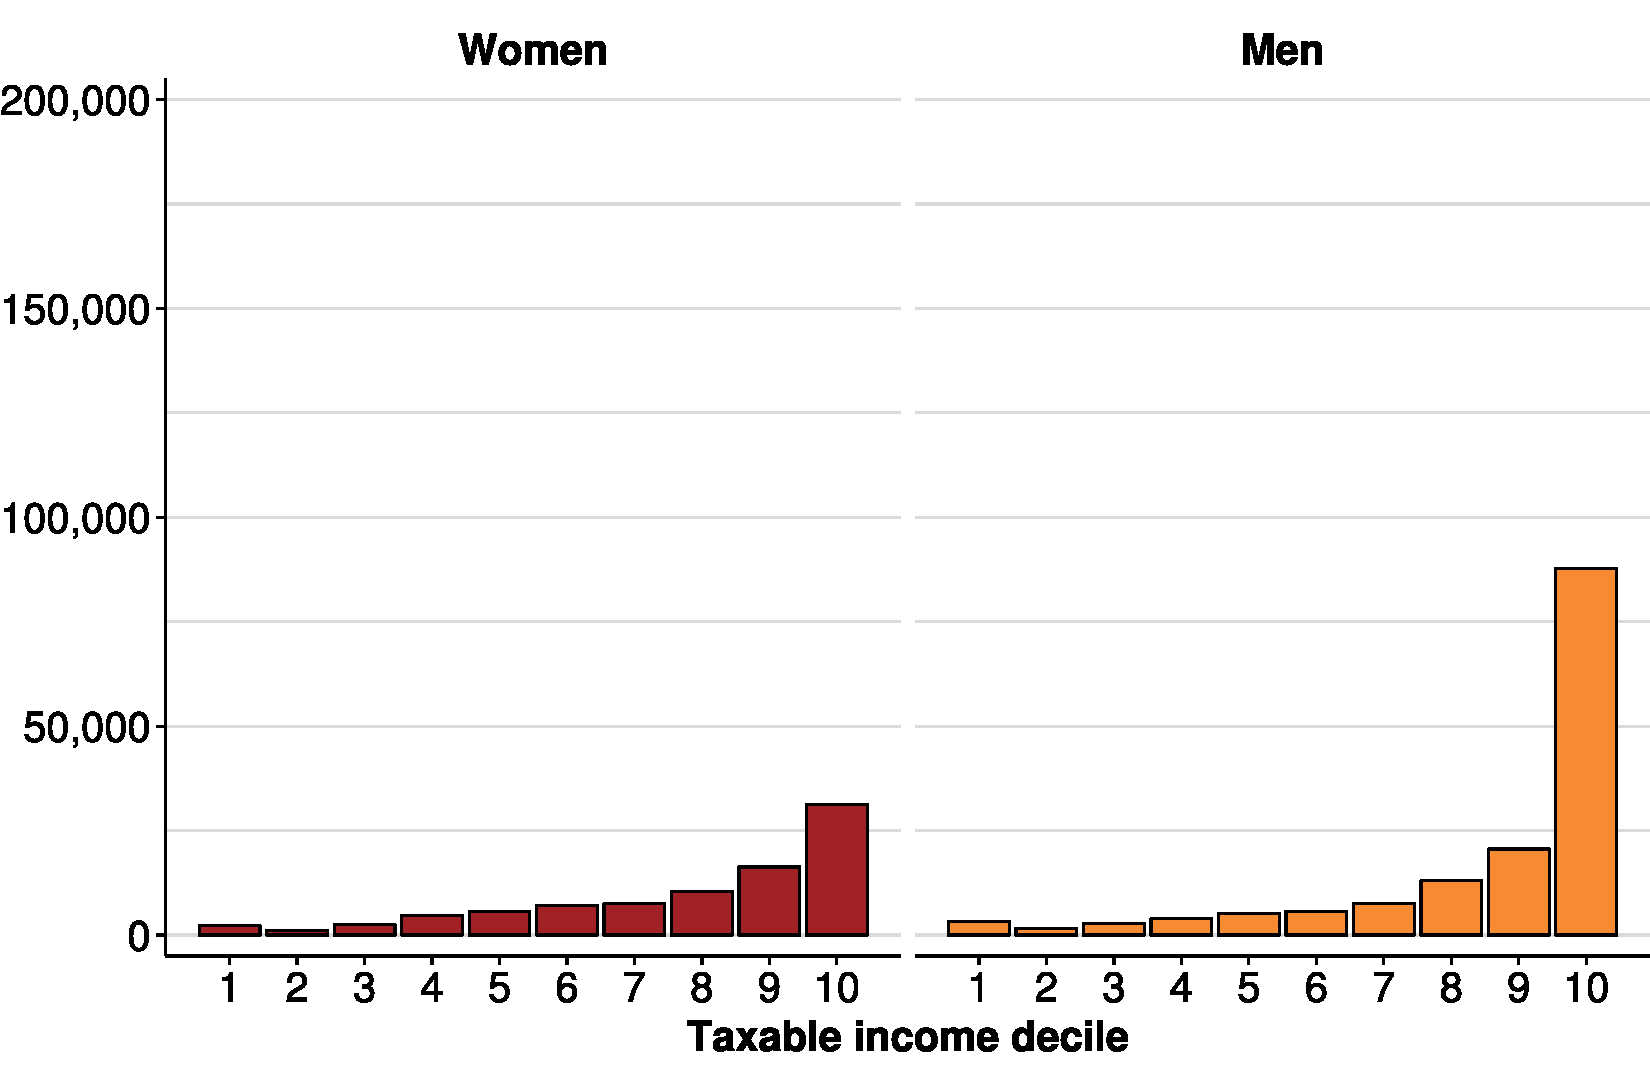
\includegraphics[width=4.47222in,height=2.94759954545455in]{atlas/n-individuals-by-decile-over-500k-and-over-25k-201718-1} 

\end{knitrout}
\noteswithsource{See \Cref{fig:pre-tax-contributions-25k-by-decile-201718}.}{Grattan analysis of \textcite{ATO2016SampleFile1314}.}
\end{figure}

The primary beneficiaries of these “catch up” provisions are likely to be younger high-income earners, overwhelmingly men. 
Typically, only high-income earners have enough disposable income to be able to afford to save more than the new \$25,000 cap on pre-tax super contributions. 
As incomes rise in the middle of a continuous career, high-income earners will be able to start saving more than \$25,000 a year. 
Provisions designed to help women and others with broken work histories will primarily help men with secure careers to get even further ahead. 

If the carry forward provisions nevertheless remain, they should be more tightly targeted to those with broken careers. For example, they might be limited to those who have worked part-time in the previous five years and restricted to those with lower super balances, such as \$300,000.\footcite{DaleyCoates2016-theConvo-Super-changes-could-benefit-rich} %

% \begin{figure*}
% \begin{minipage}[t]{\columnwidth}
% \Caption{Pre-tax super contributions of more than \$25,000 a year will likely be made mainly by rich men \dots}%
% {Projected number of individuals in 2017-18 making pre-tax contributions of more than \$25,000}%
% {fig:pre-tax-contributions-25k-by-decile-201718}
% <<n-individuals-contr-over-25k-by-decile-201718>>=
% sample_file_1718 %>%
%   apply_super_caps_and_div293() %>%
%   arrange(Gender, Taxable_Income) %>%
%   mutate(Gender = if_else(Gender == 0, "Male", "Female"), 
%          `Taxable income decile` = ntile(Taxable_Income, 10)) %>%
%   .[concessional_contributions > 25e3] %>%
%   group_by(Gender, `Taxable income decile`) %>%
%   summarise(n_persons = sum(WEIGHT), 
%             max_income = max(Taxable_Income)) %>%
%   ungroup %>%
%   {
%     grattan:::chart_data(.)
%     grplot(., aes(x = `Taxable income decile`, y = n_persons, fill = Gender)) + 
%       geom_bar(stat = "identity") + 
%       scale_y_continuous(label = comma, limits = c(0, 200e3)) +
%       scale_x_continuous(breaks = c(1:10),
%                          labels = c(1:10)) + 
%       facet_grid(~ Gender) + 
%       theme(axis.ticks.x = element_line(color = c("black", "black")))
%   }
% @
% \noteswithsource{Assumes pre-tax contributions grow at the rate of wage growth. if (TRUE || inflate_contr_match_ato) "Contributions inflated in sample file to match aggregates." else "Contributions not inflated (left as is) in sample file."}{\textcites{ATO2016SampleFile1314}{R-grattan}}
% \end{minipage}
% \hfill
% \begin{minipage}[t]{\columnwidth}
% \Caption{\dots\ and allowing taxpayers to carry forward unused caps will mainly help wealthier men}%
% {Projected number of individuals in 2017-18 with super balances of less than \$500,000 and making pre-tax contributions of at least \$25,000}%
% {fig:n-individuals-by-decile-over-500k-and-over-25k-201718}
% <<n-individuals-by-decile-over-500k-and-over-25k-201718>>=
% sample_file_1718 %>%
%   mutate(`Taxable income decile` = ntile(Taxable_Income, 10)) %>%
%   apply_super_caps_and_div293() %>%
%   filter(MCS_Ttl_Acnt_Bal < 500e3, concessional_contributions > 25e3) %>%
%   arrange(Gender, Taxable_Income) %>%
%   mutate(Gender = if_else(Gender == 0, "Male", "Female")) %>%
%   group_by(`Taxable income decile`, Gender) %>%
%   summarise(y = sum(WEIGHT)) %T>%
%   {grattan:::chart_data(.)} %>%
%   grplot(aes(x = `Taxable income decile`, fill = Gender, y = y)) + 
%   geom_bar(stat = "identity") + 
%   facet_grid(~Gender) + 
%   scale_x_continuous(breaks = 1:10, labels = 1:10) + 
%   scale_y_continuous(label = comma, limits = c(0, 200e3)) # retain scale
% @
% \end{minipage}
% % \noteswithsource{See \Cref{fig:pre-tax-contributions-25k}}{\textcites{ATO2016SampleFile1314}{R-grattan}}
% \end{figure*}




\chapter{{Proposed reforms to earnings tax breaks}}\label{chap:proposed-reforms-to-earnings-tax-breaks}

\section{The \$1.6~million cap on tax-free super earnings in retirement improves targeting}\label{sec:the-1.6-million-cap-on-tax-free-super-earnings-in-retirement-improves-targeting}
For most people, income earned by their superannuation account is taxed at 15 per cent, and capital gains earned by the account at 10~per cent. 
Once people turn 60 and retire, they can move their superannuation accounts into pension phase, and then pay \emph{no} tax on the earnings.\footcite[][13]{DaleyCoatesWoodEtAl2015Super} 
The tax-free status of super earnings in retirement is a carry-over from a world in which most superannuation withdrawals were taxed.\footnote{See footnote~\ref{footnote:Simple-super-reforms} on \cpageref{footnote:Simple-super-reforms}.}

The Government’s 2016 Budget proposes to tax some of the earnings of very large superannuation accounts in pension phase. 
The proposal would only allow retirees to transfer \$1.6~million into tax-free pension accounts.\footcite[][25]{BudgetPapers201617} %  
Any superannuation balance above this threshold would remain in the “accumulation phase” where 15~per cent tax is paid on earnings. 
The proposal is expected to save \$750~million a year by 2019-20, and much more going forward.\footcite[][25]{BudgetPapers201617}
The \ALP{} also supports this change,\footcite{Bowen-2016-Labors-plan-for-super-not-retrospective}  having previously proposed a variant of this policy that would tax annual super earnings in excess of \$75,000 at 15~per cent.\footcite{ALP2015FairerSuper} 

The \$1.6~million cap on tax-free super balances in retirement would better target earnings tax breaks towards the purpose of the superannuation system.
Tax-free super earnings are a poor way to boost the retirement incomes of low and middle-income Australians.
Previous research by Grattan Institute showed that tax breaks for superannuation fund earnings are especially poorly targeted.
Two-thirds of superannuation earnings tax concessions for those aged over 60 go to the 20 per cent whose annual incomes are above \$87,000.%
\footcite[][60]{DaleyCoatesWoodEtAl2015Super} %
The cost of tax-free super earnings for retirees is \$2.7~billion a year, and will grow as more people retire with larger super balances.

The change affects only 60,000~people, all of whom are among the wealthiest 10~per cent of people aged over~60.\DEVIATION{footnote}\footnote{\label{footnote:n-affected-earnings-tax-in-retirement}%
  Grattan analysis of \textcite{ABS-SIH11-CURF}, as per \Cref{fig:super-earnings-for-60yo-in-drawdown-phase-201718}. % 
  This estimate accords with that made by \textcite{PBO-2015-Leyonhjelm-super-costing} suggesting 60,000 people would be affected by a proposal to tax super earnings in retirement exceeding \$75,000 a year at 15~per cent in 2017-18, which would affect super accounts exceeding \$1.5~million assuming a 5 per cent rate of return. 
  \textcite{ATO2016SampleFile1314} suggests up to 98,000 taxpayers aged 60~years and over had super balances exceeding \$1.6~million in 2013-14, 
  around one-third of whom would be yet to retire in 2017-18 and would thus be unaffected by the proposed earnings tax. 
  While some self-funded retirees may not submit personal income tax returns (since super withdrawals are tax-free), most retirees with balances exceeding \$1.6~million have significant other savings outside of super, and are therefore likely to submit returns. \textcite[][28]{DaleyCoatesWoodEtAl2015Super}.% 
}   This group typically has more assets outside than inside super.\footcite[][28]{DaleyCoatesWoodEtAl2015Super}  
Their assets disqualify them from getting a pension as \$1.6~million~in super exceeds the asset limit that will apply from 2017 for a part Age Pension -- \$541,250 for a single, or \$814,250 for a home-owning couple.\footcite{DHS-2016-Asset-test}

Some argue that a \$1.6~million cap on tax-free super earnings will be too low to provide adequate income in retirement.\footcite{McCrann-scott-morrison-super-changes-big-positive-deal}  
But the \$1.6~million cap is not a restriction on the amount of super that can be accumulated, it is merely a limit on the amount retirees can have before paying \emph{any} tax on their super earnings. %
Those affected would pay only a fraction of their total income in tax (\Vref{fig:super-earnings-for-60yo-in-drawdown-phase-201718}). 
For example, someone with \$2~million of assets in super would only pay \$3000~a year in tax. 

Given the tax-free threshold outside of super, a single retiree can have a combined \$2.2~million in assets in and outside the superannuation system before they pay a cent of tax.\footnote{Accounting for the tax-free threshold, Low Income Tax Offset, and the Seniors and Pensioners Tax Offset (only available to Australians aged 65 years and over).}  
The super industry itself believes that a \$545,000 asset balance is enough to provide a home-owning single person with a comfortable retirement, or \$640,000 for a couple.\footcite{ASFA2015} 

\begin{figure}
\captionwithunits{The 15 per cent earnings tax on super balances of more than \$1.6~million will only affect high-income earners\label{fig:super-earnings-for-60yo-in-drawdown-phase-201718}}%
{Average superannuation earnings for 60+ year olds in drawdown phase, 2017\nobreakdash-18 projection}%
\begin{knitrout}
\definecolor{shadecolor}{rgb}{0.969, 0.969, 0.969}\color{fgcolor}
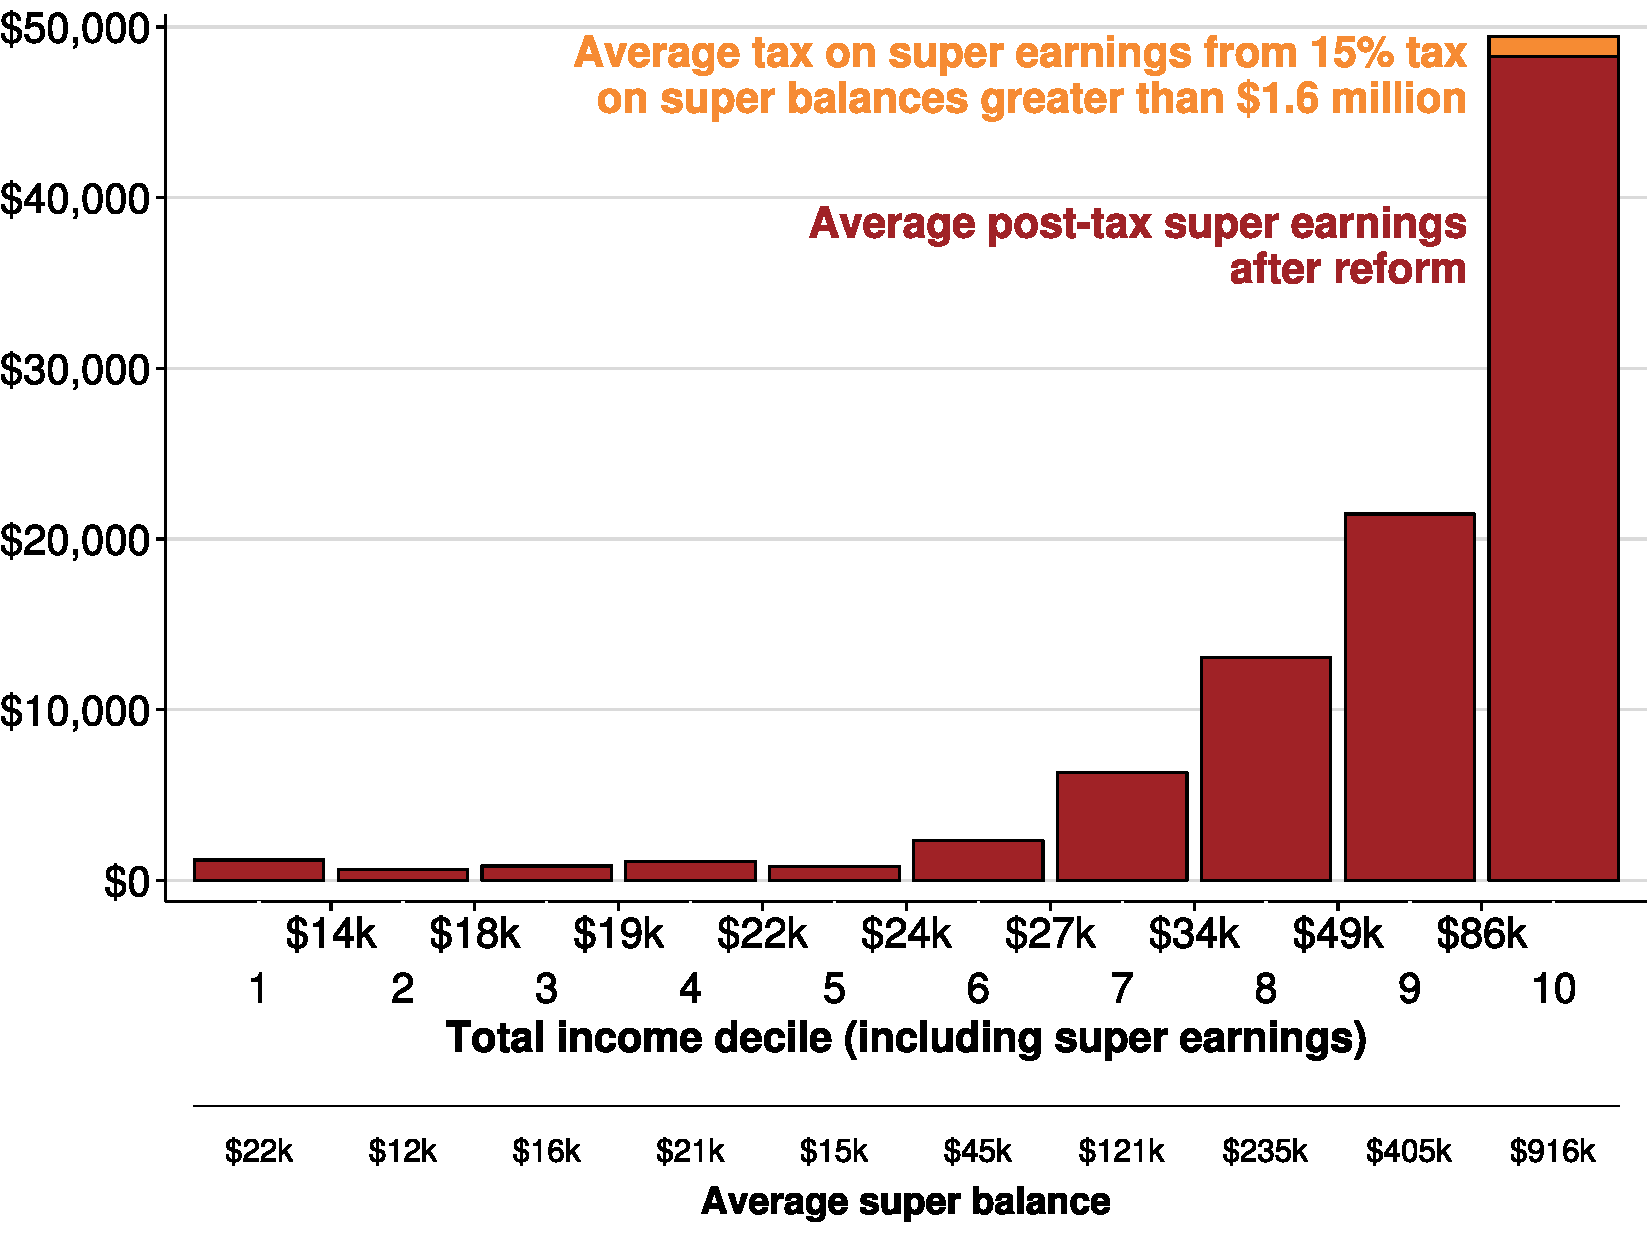
\includegraphics[width=4.47222in,height=3.38973947727273in]{atlas/15pc-tax-free-earnings-noQC-1} 

\end{knitrout}
\noteswithsource{Total income includes estimated earnings on super account balances but
excludes withdrawals. Around 70 per cent of those with super balances aged
over 60 are in pension phase, and therefore benefit from tax-free super earnings.
The impact of super earnings tax in pension phase is calculated on the basis that
taxing earnings would lead to a net increase in the effective tax rate on super
earnings of 14 per cent, from a small negative effective tax rate (given
refundable imputation credits and the capital gains tax discount), to an effective
tax rate of between 8 and 10 per cent. Individual super account balances from
the ABS Survey of Income and Housing 2011-12 are inflated to reflect the total
value of Australian superannuation fund assets as of March 2016, while
maintaining the same distribution of super account balances by age and income
reported in the ABS Survey of Income and Housing 2011-12.}%
{\textcite{ABS-SIH11-CURF}.}
\end{figure}




\phantomsection\label{para:discussion-retrospectivity}
Nor can the Government's proposed changes be labelled retrospective. 
Retrospectivity is a legal concept that applies if government changes legal liabilities for things that happened in the past.%
\footnote{%
  \textcite[][399]{Pearce-Geddes-Statutory-interpretation-2014} note that legislation is only retrospective in effect if it provides that at a past date the law is taken to have been that which it is not. None of the changes to superannuation tax breaks announced in the 2016-17 Budget alter tax law in this way.  
  See also: \textcites{ABC-Fact-check-super-changes-retrospective}{Stewart-Ingles-2016-debate-are-super-changes-retrospective}{theOz-Creighton-2016-Super-changes-reasonable-not-retrospective}{Hutchens-2016-super-changes-seriously-good}.}
The proposed \$1.6~million cap on tax-free super earnings in retirement does not change the tax treatment of past super earnings. 
Rather, the change will only affect the taxes paid on future super earnings.

Lots of changes affect investments made in the past, and no-one suggests they are retrospective. 
For instance, taxpayers purchasing shares today expect the future earnings will be subject to marginal rates of personal income tax. But if marginal rates of income tax change, they do not expect the old rates to be grandfathered to apply to all future earnings on those shares. %
Rather, they expect the earnings to be taxed at the prevailing marginal tax rate that applies at the time the income is earned.\footcite{Daley-theConvo-Retrospective-super-claim-furphy}  

This is the appropriate analogy for proposed changes to the tax treatment of earnings of superannuation accounts in excess of \$1.6~million. 
The mere fact that no tax was paid on earnings in the past does not imply that earnings in the future are entitled to be tax-free. 


Grandfathering the tax-free status of accounts for existing retirees might be politically expedient, but it is neither prudent nor fair.
Grandfathering would mean that the reform would contribute little to the budget for many years.
It would also exacerbate the intergenerational transfers of the existing tax breaks -- younger generations would continue to fund generous tax benefits that they will never be able to access.%
\footcite[][47]{DaleyWoodWeidmannEtAl2014}

\section{Taxing earnings while in Transition to Retirement improves targeting}\label{sec:taxing-earnings-while-in-TTR}
Transition to Retirement (\TTR{}) pensions allow people to move their superannuation into the “pension phase” even though they are still working. 
They can then start withdrawing from their superannuation, and they also cease to pay tax on the earnings. 

The Government plans to start taxing the earnings on super for those drawing \TTR{} pensions. 
Those withdrawing money from their superannuation, but also working and contributing to superannuation, will pay 15~per cent tax on the earnings of their super fund -- just like everyone else who is still working.

\TTR{} pensions, introduced in 2005, were supposed to encourage people to keep working part-time rather than stopping work entirely.
Yet in practice it is mainly high-wealth individuals who use these pensions to reduce their tax bills while they continue to work full-time.%
\footcite{ProductivityCommission2015SuperPolicyPostRetirement} %
In particular, \TTR{} pensions are used to enable people to stop paying tax on the earnings of accumulated super balances from a younger age while still working. 
An older Australian with a superannuation balance of \$500,000 can use a \TTR{} pension to reduce her tax paid by up to \$40,000 over five years.%
\footcite{Daley-Coates-theConvo-TaxFree-Super-Intergen-theft} %
If her superannuation balance is higher, the tax benefit is proportionately larger.

\TTR{} pensions bear little resemblance to the new explicit objective of superannuation.
These pensions and their tax breaks don't encourage additional saving, 
and do little in practice to delay retirement.
Instead they are part of an age-based tax system that allows older Australians to pay less income tax than younger Australians with similar incomes.
Abolishing access to tax-free super earnings for those using \TTR{} pensions is a positive step.\footnote{%
Other age-based provisions in our personal income tax system provide those aged over 65 with a higher income tax-free threshold (through the Seniors and Pensioners Tax Offset), a higher threshold free of Medicare Levy, and a larger private health insurance rebate.%
} %

The lack of any coherent purpose for \TTR{} pensions is reflected in the confusion about how many people will be affected by the Government’s changes. 

The Government argues that the change to \TTR{} pensions will affect 115,000 people.\footcite{TurnbullMorrison-2016-doorstop-115k-affected-by-super} %
It cites Productivity Commission analysis showing just 5 per cent of superannuants aged between 55 and 64 were drawing on their superannuation while still working.%
\footcite[][144]{ProductivityCommission2015SuperPolicyPostRetirement}

In contrast, the Association of Superannuation Funds of Australia (\ASFA{}) has suggested that the change to \TTR{} pensions could affect up to 550,000 people.%
\footnote{\textcite{ASFA-2016-Individuals-affected-by-budget-measures}. %
Although \ASFA{} noted that the number of people affected might be less than the number of accounts, this disclaimer was not reflected in its headline numbers, and was unsurprisingly not reflected in media reporting: see \eg~\textcites{Carney-2016-theHeraldSun-Super-debate-nobody-can-be-frank}{AFR-2016-Election-Super-changes-to-hit-1-3M}.}

\phantomsection
\label{ASFA-estimate-of-TTR-misleading}
Yet the Association's estimate is misleading in several ways. 
First, it relied on \APRA{} data which overstated the number of \APRA{}-regulated superannuation accounts in \TTR{} phase\@. 
\APRA{} has since revised its data and
now reports that only 148,000 \APRA{}-regulated super fund \emph{accounts} were in \TTR{} phase as at June 2015.\footcite{APRA-2016-Super-stats-pension-member-profile}
Together with an estimated 80,000 self-managed super fund accounts in \TTR{} phase,\footnote{Grattan analysis of \textcites{ATO2014e}{ATO-SMSF-2015}. Our estimate of 80,000~SMSF account holders affected by the \TTR{} pension change accords with Government estimates cited in \textcite{Crow-2016-Election-2016-ODwyer-Super}.} no more than 230,000~super accounts could be affected by the proposed change to \TTR{} pensions, far less than the 550,000 suggested by the Association. 

Second, the Association's estimate confuses the number of \TTR{} \mbox{\emph{accounts}} with the much lower number of \emph{people} affected. 
Australians on average have two superannuation accounts.%
\footcite[][13]{MinifieSavageCameron2015} %
Further, as is well known in the super industry, many people using \TTR{} pensions have many more than two accounts in order to maximize the tax advantages.%
\footnote{For example see \textcites{Superfund-wholesale-strategy--multiple-SMSF-pension-accounts}{Superfund-multiple-pension-accounts}: 
an older worker can minimise the tax paid on the earnings of contributions made while in \TTR{} by rolling the newly contributed balance into a new account each year.}
Therefore the estimated 230,000 super accounts affected belong to far fewer than 230,000 people. 

Third, many of these accounts belong to people who have fully retired, but haven't told their super fund to reclassify their pension.
They have little incentive to get their paperwork up to date, because the \TTR{} pension already provides all the benefits of tax-free super earnings to which retirees are entitled. 

Identifying the number of \emph{people} actually using \TTR{} pensions, and excluding those who could already benefit from tax-free super earnings as they are retired, we estimate that changing the tax treatment of super fund earnings for \TTR{} pensioners would affect 115,000 people,%
\footnote{We identify the number of people aged 56 to 64 (accounting for the lift in the Preservation age to 56 by 2017-18) that are drawing a super income stream while still reporting wage income, projecting forward population growth among this cohort to 2017-18 when the change will take effect.
Grattan analysis of \textcite{ABS2015-Survey-of-income-and-housing-2013-14}.} %
in line with the Government's estimate.


\chapter{{Proposed reforms to total super contributions}}\label{chap:proposed-reforms-to-total-super-contributions}
A person can contribute to super from “after tax” as well as pre-tax income. 
Such contributions can be made from other assets accumulated outside super.

\section{A \$500,000 lifetime cap on post-tax contributions improves targeting}\label{sec:the-500000-lifetime-cap-on-post-tax-contributions-is-a-big-step-forward}
The Government proposes to cap post-tax contributions at \$500,000 over a lifetime. 
The cap on post-tax contributions, which will apply to any post-tax contributions made since 2007-08.%
\footnote{\textcite{BudgetPapers201617}. The Australian Taxation Office only has reliable records on non-concessional contributions made from 1 July 2007.} %
At present post-tax contributions are capped at \$180,000 a year -- or \$540,000 over any three-year period.
This change is expected to improve the budget by \$250~million a year by 2019-20, and these savings will grow significantly over time.%
\footnote{For example \textcite{Coorey-2016-Super-cap-PBO} cites unpublished PBO costings that suggest the \$500,000 lifetime cap on post-tax contributions would raise \$5.7~billion over a decade.}
The \ALP{} supports a \$500,000 lifetime cap on post-tax contributions but only including post-tax contributions made since Budget night 2016, on the basis that a backdated cap is “retrospective”. 
This more modest change would save \$500~million less over four years than the Government’s plan.%
\footnote{The PBO estimates the \ALP{} proposal would save only \$50~million over four years. \textcite{ALP-2016-Making-super-fairer}.}






Post-tax super contributions are designed to allow individuals to make top-up payments to a superannuation fund.
Australians made \$33.6~billion in post-tax super contributions in 2012-13, about three-quarters of all voluntary contributions.\footcite[][54]{DaleyCoatesWoodEtAl2015Super} 





In reality, after-tax contributions do little to increase retirement savings.
Instead most people who make after-tax contributions already have large balances and typically contribute from existing pools of savings in order to minimise their tax (\Vref{fig:share-of-taxpayers-and-post-tax-contributions}).
Only about 1~per~cent of taxpayers have total super account balances of more than \$1~million, yet this tiny cohort makes almost one-third of all post-tax contributions.

A \$500,000 lifetime cap on post-tax contributions would go a long way to aligning super tax breaks with the purpose of superannuation. 
Those who have contributed more than \$500,000 after tax before the cap was introduced would be prevented from contributing any more. 
These people are unlikely to qualify for an Age Pension given how much they have already accumulated in super from post-tax contributions, and taking into account that they probably also have substantial pre-tax contributions, savings outside of super, and in many cases, the super balance of a second income earner if they are a dual-income household.

As well as cutting back earnings tax breaks for high-income earners, a lifetime cap would restrict so-called `re-contribution strategies' that allow people to minimise the tax paid on superannuation fund balances passed on as inheritances.%
\footcite[][54--55]{DaleyCoatesWoodEtAl2015Super}

Critics have argued the \$500,000 lifetime cap is both retrospective and too low.% 
\footcites{Chartered-accountants-on-2016-Govts-budget-super-changes}{McCrann-scott-morrison-super-changes-big-positive-deal} %
Both these claims are incorrect. \enlargethispage{-0.25\baselineskip}

\subsubsection{The proposed lifetime cap is not retrospective}
Contrary to the position of the \ALP{}, a lifetime cap is not retrospective for the same reasons that the \$1.6~million cap on tax-free super earnings in retirement is not retrospective (see \cpageref{para:discussion-retrospectivity}). 
Both changes ultimately depend on a person’s circumstances in the future, and attach liabilities to these circumstances. 

The cap on post-tax contributions only applies to additional post-tax contributions in the future. 
The Budget explicitly states that contributions made before the announcement are not affected, even where they exceed~\$500,000.\footcites{BudgetPapers201617}{Stewart-Ingles-2016-debate-are-super-changes-retrospective} %  
True, the limits take into account the amount that has already been contributed, but no adverse consequence flows from historic contributions; the change merely limits future contributions. 
To draw an analogy, legislation is not retrospective if it changes how to take into account assets accumulated in the past in order to assess future Age Pension payments. 

\subsubsection{A \$500,000 lifetime cap is not too low} 
A \$500,000 lifetime cap will not lead to a mass movement onto the Age Pension. 
Some might think that a \$500,000 super balance doesn’t sound like much. 
But it is larger than the super balance of 19~in 20 taxpayers today. 
A man aged 60~to 64 years today can expect to retire with average superannuation savings of \$292,000, and a woman with \$138,000. 
Even in a mature super system, where workers make compulsory super contributions of at least 9~per cent for their working lives, most people will retire with less than \$500,000 in super.%
% \enlargethispage*{-0.25\baselineskip}\enlargethispage*{0.25\baselineskip} 

\begin{figure}[t]
\captionwithunits{Voluntary post-tax contributions are mostly made by those who already have high superannuation balances\label{fig:share-of-taxpayers-and-post-tax-contributions}}%
{Share of taxpayers and post-tax contributions, by existing superannuation balance, 2013-14}%
\begin{knitrout}
\definecolor{shadecolor}{rgb}{0.969, 0.969, 0.969}\color{fgcolor}
\includegraphics[width=4.47222in,height=3.05076552954545in]{atlas/share-of-taxpayers-and-post-tax-contributions-1} 

\end{knitrout}
\noteswithsource{Excludes post-tax contributions made by people who do not lodge tax returns.}%
{Grattan analysis of \textcite{ATO2016SampleFile1314}.}%
\end{figure}


In any case, the value of total retirement assets is likely to be much higher than the value of post-tax super contributions.\DEVIATION{avoid typographic sin (consecutive words)}
A person making \$500,000 of post-tax contributions to superannuation will usually also be making substantial pre-tax contributions, and have large savings outside of superannuation. 
%
% In any case, total retirement assets are likely to be much larger than post-tax contributions to super. 
% A person who makes \$500,000 of post-tax contributions to super will usually also make large pre-tax contributions, and have substantial savings outside superannuation. %
Most people affected by the lifetime cap will be high-income earners whose retirement assets exceed \$500,000, making them ineligible for the Age Pension. 

The proposed lifetime cap of \$500,000 does not affect the ability of the self-employed to accrue much larger superannuation balances: no change is proposed to provisions that allow small business owners to transfer business assets of up to \$1.4~million into their superannuation fund.\footcite[][57]{DaleyCoatesWoodEtAl2015Super} 

Finally, the benefits of the current arrangements must be balanced against the costs. 
The current rules allow a very small number of people with limited assets to make catch-up contributions to super. 
There are few in this category: those with broken work histories are unlikely to start earning so much towards the end of their lives that they can afford to contribute both \$25,000 a year before tax, and more than \$500,000 after tax within a few years. 
And the improvement in their retirement incomes needs to be balanced against the much larger tax leakage that happens when a much larger number of well-off taxpayers unlikely to qualify for an Age Pension make additional post-tax contributions to minimise their tax. 


Some Coalition backbenchers have signalled their opposition to the \$500,000 lifetime cap, suggesting instead a \$750,000 or \$1~million cap.\footcite{Coorey-2016-Govt-consider-concessions-to-appease-MPs} % 
Such an increase is unjustified. 
Further, increasing the lifetime cap beyond \$500,000 may cost the budget more than the current \$180,000 annual cap on post-tax super contributions. 
Where the lifetime cap is set above the \$540,000 bring-forward rule, total post-tax contributions are likely to increase. 
Additional one-off contributions are likely to be more than the reduced contributions from those making regular post-tax super contributions year after year.\footnote{%
The PBO estimates that of those aged 55 and over in 2013-14, just 12~per cent of post-tax contributions were made by people who had contributed more than \$500,000, and only 6~per cent were made by people who had contributed more than \$800,000. \textcite{PBO2015-Super-for-retirement-not-tax-minimisation}.%
% PBO: 
% Only a relatively small proportion of individuals making regular non-concessional contributions
% would be expected to have their contributions limited by the lifetime cap. Of those aged 55 or over
% in 2013-14, just 12 per cent of non-concessional contributions were made by individuals who had
% contributed more than $500,000 and only 6 per cent were made by individuals who had contributed
% more than $800,000.
%
}  

\subsubsection{Any exemptions to the lifetime cap should be limited}
Some have called for exemptions to the \$500,000 lifetime cap on post-tax contributions in cases of divorce, or other major life events.\footcite{AFR-Super-cap-carve-outs-leave-industry-underwhelmed-2016}  
Yet any exemptions to the lifetime cap should be applied sparingly, if at all, to avoid creating further tax-planning loopholes. 

The existing superannuation rules already allow superannuation fund balances to be split between a couple who get divorced, and these transfers are not classified as super contributions by the receiving spouse.%
\footnote{See \textcites{AG-2016-Super-splitting-laws-FAQ}{ATO-2016-Super-and-relationship-breakdowns-APRA-funds}{ATO-2016-Super-and-relationship-breakdowns-SMSF-funds}.}

A more valid concern is where a super fund member, having made substantial post-tax contributions, splits their super balance with their spouse and is then unable to make additional post-tax super contributions to top up their super account balance. 
Where at least one member of a household has made post-tax contributions and the balance of any super funds is split as part of the divorce settlement, any post-tax super contributions should be split in line with the splits in super balances, also counting towards the lifetime cap of the spouse receiving the super balance. 
Any exemptions for divorce should not permit two members of a couple to contribute more after tax if they divorce than if they stay together.

Another justifiable exemption to the lifetime cap would be post-tax contributions funded by workcover compensation payouts. 
Such an exemption would recognise that workers’ compensation is made on the grounds of economic loss, reducing recipients’ future earnings and capacity to make pre-tax contributions in later years. 

In contrast, there is no case for allowing inheritances to be exempt from the lifetime cap on post-tax contributions. 
The existing super rules already permit superannuation benefits to be transferred from a deceased super fund member to a surviving spouse, and such funds are not counted towards pre- and post-tax contributions caps.%
\footnote{For example, see \textcites{ATO-2016-Super-death-benefits-APRA}{ATO-2016-Super-death-benefits-SMSF}.}   
Permitting those with inheritances to make extra post-tax contributions in excess of the lifetime cap would allow those with inheritances to make extra use of super earnings tax breaks – by making extra post-tax contributions beyond the \$500,000 limit -- if they inherit money, but not if they save it themselves.
Those receiving a windfall inheritance should not expect an extra bonus supported by other taxpayers through the superannuation system.

\subsubsection{A lifetime cap would be administratively straightforward} 

Introducing a lifetime cap is administratively straightforward. 
The \ATO{} already administers a lifetime cap, called the \CGT{} cap, on some post-tax contributions by small business owners.\footcite{ATO-2016-CGT-cap-amount} %
The Coalition's backdated cap would only apply from 2007 -- the point where information on post-tax contributions started being collected accurately.\DEVIATION{2007 not only time accurate collect} 
The \ATO{} should consider sending annual notices to taxpayers to update them on their entitlements to make post-tax contributions.

\section{Abolishing work test for super contributions encourages tax planning}\label{sec:abolishing-work-test-encourages-tax-planning}
The 2016 Budget also proposed removing the work test, a change that would allow more people aged over 65 to contribute to super even if they are not working and saving for their retirement. 
Currently, people aged 65 to 74 may only contribute to super if they pass a minimal work test of working 40~hours over 30~consecutive days in the financial year.\footcite{ATO-2016-Age-super-contr-caps} %
The \ALP{} does not support abolishing the work test.\footcite{ALP-2016-Making-super-fairer}

This change is undesirable because it does not serve the purpose of superannuation. 
Removing the work test for older Australians will do little to support genuine retirement savings, but will turbocharge tax planning for wealthy retirees. 

The existing work test is not onerous.
It requires someone to work 40~hours over 30~consecutive days in the financial year. 
If people are not passing this minimal test it is not clear they are legitimately working and saving for retirement.

If people are not working, but are contributing to super, then most of these contributions are probably sourced from retirement savings outside of superannuation -- such as shares or investment property. 
Allowing such contributions substantially reduces tax liability because investment income can be washed through the superannuation fund at a tax rate of just 15 per cent, rather than at marginal tax rates. 
Such strategies do little to boost retirement savings while imposing costs on the budget and other taxpayers. 
Abolishing the work test will open up additional tax breaks for wealthier older Australians who are already retired.

Consider the example of a retired 70-year old earning \$150,000 a year just from an investment portfolio. 
She does not work and therefore cannot contribute to superannuation under current arrangements.  
If the proposed change takes effect, she will be able to contribute \$25,000 (the new pre-tax contribution cap) into superannuation. 
On this contribution -- which is really just investment income -- she would pay contribution tax of 15 per cent instead of her marginal rate of 39 per cent. 
This would reduce her total tax bill by \$6000. 
Future earnings on the \$25,000 contributed would be tax-free. 

In addition, those not working would be able to transfer other savings as post-tax contributions into superannuation, where future earnings are either untaxed, or only taxed at 15 per cent. 
This will be a particularly attractive tax-planning opportunity if the lifetime cap on post-tax contributions is not legislated. 

\chapter{{Number of people adversely affected by changes}}\label{chap:how-many-people-will-be-adversely-affected-by-the-super-changes}

The Coalition has stated that the 2016 Budget super changes will adversely affect 4 per cent of super account holders.\footcite{BudgetPapers201617}  
The super industry, by contrast, maintains that up to twice as many super account holders -- or 1.26~million people -- will be worse off under the changes (\Vref{tbl:n-affected-by-2016-super-changes}).%
\footcite{ASFA-2016-Individuals-affected-by-budget-measures}
Our independent analysis is in line with the Government’s claims, while those of the Association appear unreliable. 

First, as noted in \Cref{sec:taxing-earnings-while-in-TTR} %
on \cpageref{ASFA-estimate-of-TTR-misleading}, 
the Association overestimates the number affected by changes to \TTR{} pensions by confusing the number of \TTR{} accounts (more than 500,000) with the number of people affected (most likely 115,000).
And many of the people affected may be eligible for tax-free super earnings anyway. 

Second, adding up the number of people separately affected by each measure, as the Association does, double-counts people affected by more than one change.
There are many overlaps. 
About a fifth of post-tax contributions are made by those with a super balance over \$2~million, and they are therefore likely to be affected by the cap on tax-free super balances over \$1.6~million %
(\Vref{fig:share-of-taxpayers-and-post-tax-contributions}). %
People who make large post-tax contributions also tend to make large pre-tax contributions,\footcite[][42]{DaleyCoatesWoodEtAl2015Super} and so will be affected by both the \$500,000 lifetime cap on post-tax contributions and the \$25,000 cap on pre-tax contributions. 

% manual columnbreak 
\vfill\eject 

The estimate for the number of people with a super account is based on the \ATO{} taxation statistics, which reconciles the approximately 30~million super accounts with the taxpayers holding the accounts. 
The estimated population includes only individuals with a Member Contribution Statement to avoid double-counting and is adjusted to reflect population growth to 2017-18.

We estimate that about 40,000 people will be affected by both the change to the \TTR{} pensions and the changes to the pre-tax contribution cap or the Division 293 income threshold.\footnote{Grattan analysis of \textcite{ABS2015-Survey-of-income-and-housing-2013-14}.} %
But a lack of publicly available data means we are unable to identify those that will affected by more than one of: the \$1.6~million cap on tax-free super earnings in retirement; the \$500,000 lifetime cap on post-tax contributions; and the tighter rules governing pre-tax contributions.%
\footnote{We estimate using data from \textcites{APRA2016-Annual-Superannuation-Bulletin-Jun2015}{ATOTaxstats201314} that 18.75~million people will have a super account by 2017-18, up from an estimated 17.5~million in 2013-14.} %

Overall, our analysis suggests that just over 4~per cent of superannuation account holders will be adversely affected by the Government's super changes -- in line with the Coalition's estimate (\Cref{tbl:n-affected-by-2016-super-changes}). 
Even so, we probably overestimate the total number affected as we cannot account for all the people affected by more than one policy change. 
We also do not account for any positive impacts from other parts of the super package that may offset the adverse effects of other Budget changes.



\begin{table*}
\caption{Estimates of the number of people adversely affected by the 2016 Budget super changes, 2017-18\label{tbl:n-affected-by-2016-super-changes}}

\begin{tabularx}{\textwidth}{lXrr}
%
\toprule
 & &\multicolumn{2}{c}{\textbf{Number of people negatively affected{\Large\strut}}} \tabularnewline
 \cmidrule(lr){3-4}
\multicolumn{2}{l}{\textbf{Policy change}} & \textbf{\ASFA{} estimate}{\Large\strut} & \textbf{Grattan estimate} \tabularnewline
\midrule
\multicolumn{2}{l}{{{Contributions tax breaks}}} &\tabularnewline
& \$25,000 pre-tax contribution cap and lower \$250,000 income threshold for Division 293 tax & 500,000 & 520,000\tabularnewline
& Remove anti-detriment provision in respect of death benefits from superannuation & 20,000 & 20,000\tabularnewline[5pt]
\multicolumn{2}{l}{{{Earnings tax breaks}}} &\tabularnewline
& \$1.6~million cap on tax-free earnings in retirement & 110,000 & 60,000\tabularnewline
& Abolish tax-free super earnings for Transition to Retirement pensions & 550,000 & 115,000\tabularnewline[5pt]
\multicolumn{2}{l}{{{Rules governing total super contributions }}} &\tabularnewline
& \$500,000 lifetime cap on post-tax contributions & 80,000 & 80,000\tabularnewline[5pt]
\multicolumn{2}{l}{\emph{{Less those affected by more than one policy change}}} & \emph{{0}} & \emph{{40,000}} \tabularnewline[5pt]
\multicolumn{2}{l}{\textbf{Total negatively affected by package}} & \textbf{Up to 1,260,000} & \textbf{Up to 755,000}\tabularnewline[5pt]
\cmidrule(lr){3-4}
\multicolumn{2}{r}{Number of people with a super account} & 14,000,000 & {18,750,000} \tabularnewline[5pt]
\multicolumn{2}{r}{\textbf{Proportion of superannuants affected}} & \textbf{Up to 9.0\%} & \textbf{Up to 4.2\%} \tabularnewline
\bottomrule
\end{tabularx}
\noteswithsource{We adopt \ASFA{}'s estimates of the number of people affected by the lifetime cap on post-tax contributions and abolition of anti-detriment provisions in the absence of publicly available data. 
Our estimate of those affected by reforms to \TTR{} pensions is consistent with that of the Productivity Commission.
Our estimate of the number of people affected by the cap on tax-free earnings in retirement is consistent with \textcite{PBO2015-Super-for-retirement-not-tax-minimisation} and \textcite{ATO2016SampleFile1314}, as discussed in footnote~\ref{footnote:n-affected-earnings-tax-in-retirement} on \cpageref{footnote:n-affected-earnings-tax-in-retirement}. %
Our estimate of the number of people affected by more than one policy change is likely to be an underestimate, and hence the total number affected by any one measure in the super package will be overestimated, due to data limitations. 
Our estimate of the number of superannuation accounts is based on ATO data on the number of people with a superannuation fund plus population growth using ABS population projections. It excludes individuals without a Member Contribution Statement to avoid double-counting.
}%
{\textcites{ASFA2015}[][Vol.~2, p.\ppspace 144]{ProductivityCommission2015SuperPolicyPostRetirement}{ABS2013t}{ATO2016SampleFile1314}[][13]{MinifieSavageCameron2015}.}%
%
\end{table*}


\chapter{Contribution to budget repair}\label{chap:contr-to-budget-repair}
The Government’s super package will make a significant contribution to budget repair, which will grow over time as super matures and the population ages. 
Measures that reduce the earnings tax breaks to high-income earners – especially the \$1.6~million cap on tax-free super earnings in retirement and the \$500,000 lifetime cap on post-tax contributions -- will reduce the budgetary cost of super tax breaks in the long-term, which have become unsustainable. 
Importantly, these changes will have little or no impact on future Age Pension expenditures, since they overwhelmingly affect high-income earners who are unlikely to ever qualify for the Age Pension in retirement.\footcite[][29]{DaleyCoatesWoodEtAl2015Super}

Yet despite including measures which reduce superannuation tax breaks by \$2.6~billion a year by 2019\nobreakdash-20, the annual budget savings from the Government’s super proposals only total \$0.775~billion in 2019\nobreakdash-20 (\Vref{fig:net-contr-to-budget-repair}). 
This is because widely publicised cuts to super tax breaks for high-income earners are offset by measures that widen access to super tax breaks to other groups. 
Retaining the \LISTO{} is expected to cost the Budget \$800~million a year by 2019\nobreakdash-20. 
Permitting all taxpayers to contribute directly to their super fund and claim a deduction on their personal income tax return will cost a further \$750~million. 

\begin{figure}
\captionwithunits{The Government’s super package will save less than \$1~billion a year once fully implemented\label{fig:net-contr-to-budget-repair}}%
{Net budget impact of super package components, 2015-16 to 2019-20 (billions)}
% Warning due to stacked bar (ok)
\begin{knitrout}
\definecolor{shadecolor}{rgb}{0.969, 0.969, 0.969}\color{fgcolor}
\includegraphics[width=4.47222in,height=2.94759954545455in]{atlas/net-contr-to-budget-repair-1} 

\end{knitrout}
\noteswithsource{Fiscal savings are as reported in the 2016-17 Budget. Extending the income threshold for the low-income spouse tax offset is included in the `contributions tax expansion' series.}{\textcite{BudgetPapers201617}.}
\end{figure}

Other measures to expand contributions tax breaks -- measures that should not proceed because they do little to support the purposes of super -- reduce the budgetary savings from the Government’s super package by a further \$305~million a year (\Vref{tbl:Summary-table}). 

In particular, allowing people to carry forward unused pre-tax contribution caps to future years is expected to cost \$250~million by 2019\nobreakdash-20, and more over time.%
\footnote{%
The government estimates the measure will only cost \$350~million over the four years to 2019-20. 
However, since taxpayers will only be able to carry forward the unused portion of their contributions cap from 1 July 2017 onwards, the full cost of the policy change will only become apparent from 2021-22 onwards, when individuals have access to unused caps over the previous four years. 
\textcite{DaleyCoates2016-theConvo-Super-changes-could-benefit-rich}
} %
If these changes do not proceed, the budgetary savings from the government’s package would be boosted to about \$1~billion a year in total. 

The \ALP{} is proposing reforms that would do more to repair the budget than the Government’s plan. 
The \ALP{}’s super package would raise \$2.1~billion a year, or  \$1.3~billion a year more than Government’s proposal (\Cref{tbl:Summary-table}). 
If the Government makes “concessions”, they will mostly improve the budget position. 
In contrast, many amendments to the government’s package advocated by industry groups, such as watering down the limits on super tax breaks for high-income earners that don’t need them, could easily result in a package that makes the budget position worse overall. 

\chapter{Future changes\label{chap:future-changes}}
Overall, both the Government’s and the \ALP{}’s proposed changes are a big step in the right direction. 
Those affected are overwhelmingly high-income earners who are unlikely to ever qualify for the Age Pension in retirement. 
Yet the changes don’t go far enough.

\section{Super tax breaks remain poorly targeted overall even after 2016 Budget reforms}\label{sec:super-tax-breaks-remain-poorly-targeted-overall-even-after-2016-budget-reforms}

Even after the reforms, super tax breaks will overwhelmingly flow to high-income earners who do not need them. 
People in the top 20 per cent of income earners, who are unlikely to ever get a pension, will still receive about half of all super pre-tax contribution tax breaks.

Treasury projections in the 2016 Budget show that the lifetime value of tax breaks to high-income men remains much higher than the value of the Age Pension for low-income earners, even after the Government's Budget changes (\Vref{fig:npv-total-govt-lifetime-support-through-Age-Pension-super-tax}). % 
These projections are likely to be conservative since they ignore all post-tax super contributions, which are largely made by high-income earners, boosting the super earnings tax breaks they receive.\footnote{Different assumptions about life expectancy and draw down rates can also result in much higher estimates of the lifetime benefits to high-income earners. For example, \textcite{Industry-Super-2015-Off-target-current-settings} calculates that superannuation tax breaks for the top 5 per cent of income earners are worth more than \$2~million for men over their lifetimes.}

\begin{figure}%[!b]
\captionwithunits{Lifetime income support is unequally distributed even after the Government's changes\label{fig:npv-total-govt-lifetime-support-through-Age-Pension-super-tax}}%
{Net present value of total government support over a lifetime through the Age Pension and super tax breaks in 2016}%


% Warning = FALSE for font family spurious warning
\begin{knitrout}
\definecolor{shadecolor}{rgb}{0.969, 0.969, 0.969}\color{fgcolor}
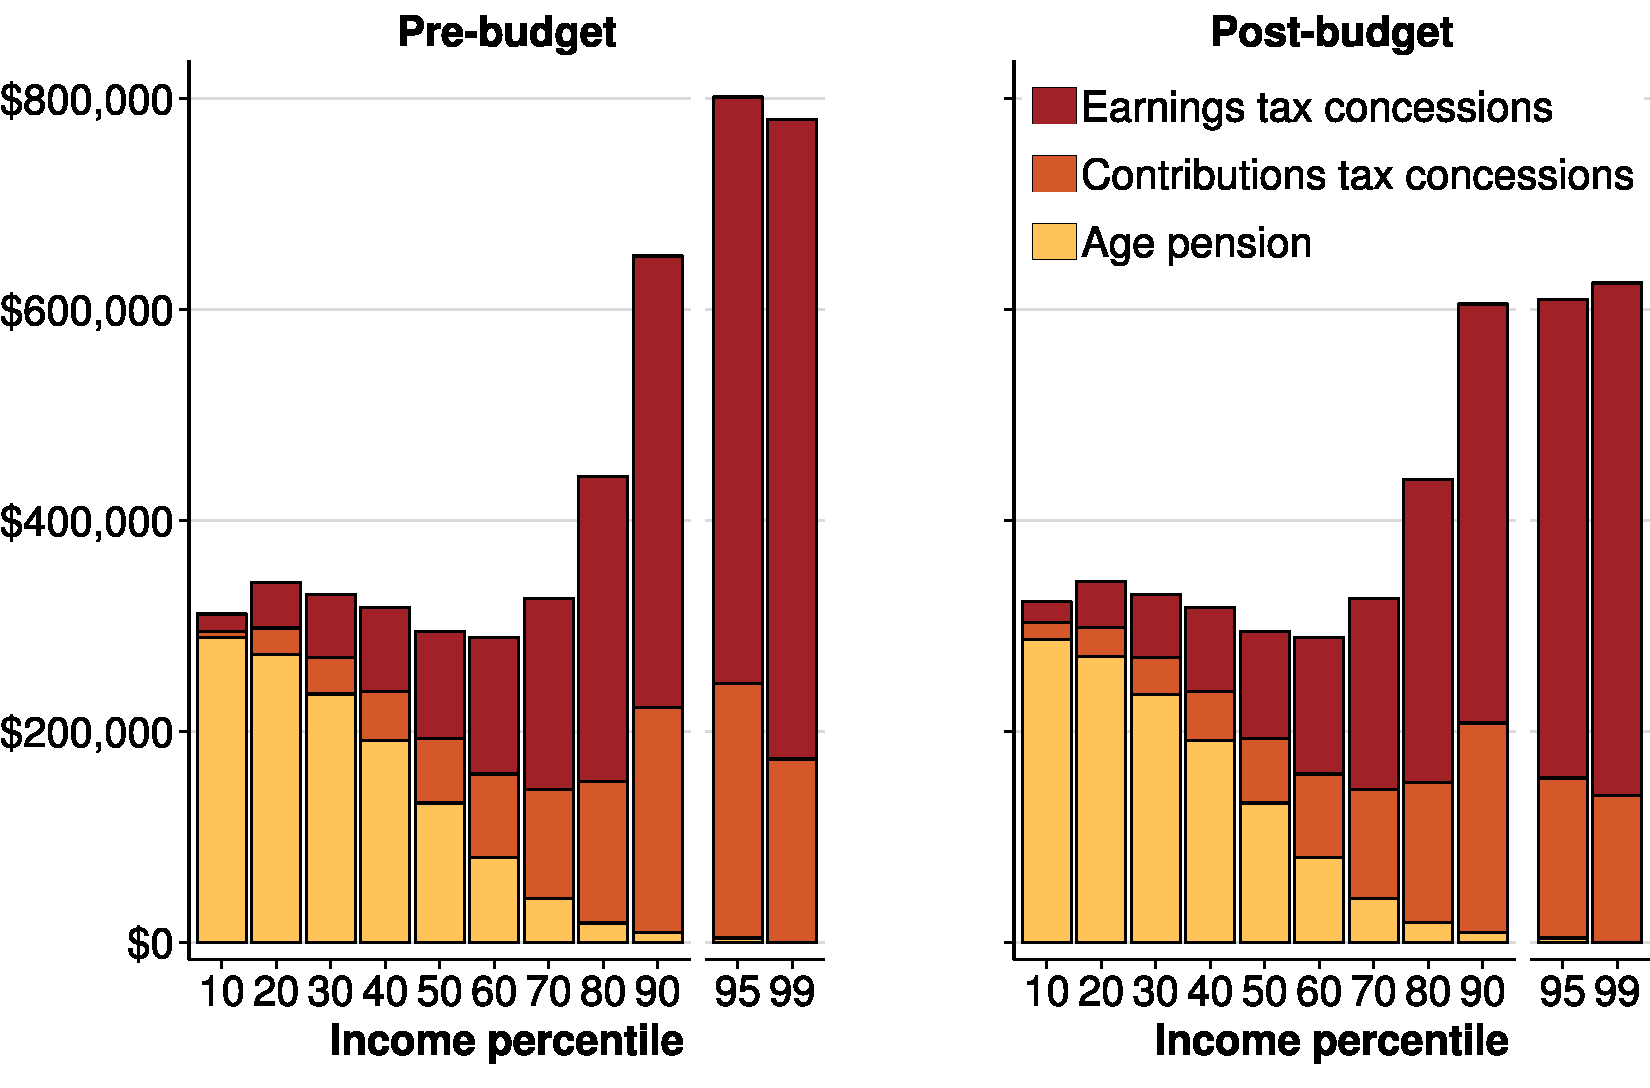
\includegraphics[width=4.47222in,height=2.94759954545455in]{atlas/npv-total-govt-lifetime-support-throught-Age-Pension-super-tax-cowplot-1} 

\end{knitrout}


% {Individuals are assumed to commence work in 2016 at age 30 and work until age 70, with a predicted life expectancy of 92.
% Accumulated superannuation benefits are invested in an account-based pension and individuals are assumed to draw down their assets at the current age based minimum drawdown rates.
% The level of tax assistance and Age Pension entitlements are discounted by 5 per cent per annum to calculate a net present value in 2016 dollars.
% Annual incomes are calculated for each percentile based on the distribution of earners at each single year of age.
% Assumes no non-concessional contributions}%
\noteswithsource{Individuals are assumed to commence work in 2016 at age 30 and work
until age 70, with a predicted life expectancy of 92. Accumulated superannuation
benefits are invested in an account-based pension and individuals are assumed
to draw down their assets at the current age-based minimum drawdown rates.
The level of tax assistance and Age Pension entitlements are discounted by 5
per cent per annum to calculate a net present value in 2016 dollars. Annual
incomes are calculated for each percentile based on the distribution of earners at
each single year of age. Assumes no post-tax contributions.}%
{\textcite[][4]{Budget-2016-17-Super-fact-sheets}.}
\end{figure}

Before the changes, someone in the top 1 per cent of income earners could expect to receive \textbf{two-and-a-half times as much} in tax breaks from super over her lifetime as a retiree with no assets receives in pension. 
This is also two-and-a-half times as much as the average income earner receives in pension and super tax breaks combined. 
The Budget changes merely trim the worst of these excesses: the top one per cent now receives \textbf{just twice as much} as low or average income earners.

There is no public consensus on how government support for people's retirement should be distributed. 
Yet when self-funded retirees receive twice as from government as the assistance provided by the pension, it is clear more work is required to align super tax breaks with their policy purpose.

\section{Opportunities to improve targeting of super tax breaks }\label{sec:opportunities-to-improve-targeting-of-super-tax-breaks}

Changes to superannuation in the past have been too timid. The 2016 Budget changes will not end the need for reform. In 2019\nobreakdash-20, the Government's package will trim \$775~million a year from super tax breaks, just 2 per cent of their overall value.

Even if the Budget reforms are implemented, a wide gap will remain between the purpose of the system and what it delivers. 
Decisive reform must target superannuation tax breaks at those who need them most.

Grattan Institute's recent \citetitle{DaleyCoatesWoodEtAl2015Super} report identified three reforms to better align tax breaks with the goals of superannuation, and would go much further than the government’s package.\footcite{DaleyCoatesWoodEtAl2015Super}

\textbf{Contributions from pre-tax income should be limited to \$11,000 a year}. 
Such a change to create a much more targeted system would primarily affect the top 20 per cent of income earners, but they would still have a comfortable retirement, mostly without an Age Pension. 
The change would improve budget balances by \$3.5~billion a year. 
If the income threshold for Division 293 tax were lowered to \$250,000 as the government proposes, or \$200,000 as proposed by the \ALP{}, pre-tax super contributions could instead be capped at \$15,000 a year.
This would ensure those on upper middle incomes would still make sufficient contributions -- after paying tax on those contributions -- to be unlikely to qualify for an Age Pension in retirement. 

\textbf{Lifetime contributions from post-tax income should be limited to \$250,000.} 
While a lifetime cap on post-tax contributions is a sensible step, the \$500,000 cap is too high. 
The cap might not sound like much to some, but it is more than what 95 per cent of taxpayers have in super right now. 
A lifetime limit of \$250,000 (in addition to pre-tax contributions) is likely to be more than most people with broken work histories can afford to contribute to super. Beyond this point, post-tax contributions are much more likely to be tax planning than catch-up.

\textbf{\emph{All} earnings in retirement should be taxed at 15 per cent}, the same as superannuation earnings before retirement. 
The proposed \$1.6~million super balance cap, while a positive step, is far too high. %
Allowing retirees to amass four times the amount needed for a comfortable retirement and not pay a cent of tax is unacceptable. 
Even people affected by the cap will pay very little extra tax compared to their total income.

Imposing a 15 per cent tax on all superannuation earnings in retirement would have little impact on retirement incomes.\footcite[][63]{DaleyCoatesWoodEtAl2015Super} 
Those with super but on low to middle incomes could maintain a zero tax rate on earnings by moving savings out of super. 
Their total taxable earnings would be below the tax-free threshold, which is effectively around \$30,000 for those aged over 65 who qualify for the Seniors and Pensioners Tax Offset (\SAPTO{}). 
A 15 per cent tax on all super earnings would improve budget balances by \$2.7~billion a year today, and much more in future.

These changes would help fix the budget without compromising the objectives of the superannuation system. 
They would also be fair. 
Low-income earners and younger people would pay less in other taxes if super tax breaks for the wealthy were wound back. 
Those already retired would pay some tax on their superannuation savings but they would pay much less tax than wage earners on similar incomes. For a small proportion of women with higher incomes later in life, the changes would reduce their catch-up contributions. 
Yet the changes would reduce the tax breaks far more for those with substantial means to save for their own retirement without government support.

\subsection{Broader reforms to Australia's retirement incomes system are also needed}\label{broader-reforms-to-australias-retirement-incomes-system-are-also-needed}

Many other features of Australia's retirement incomes system also need reform, and could contribute to the task of budget repair. Areas beyond the scope of this paper include:

\begin{itemize}
\item
  Increasing the age at which tax-free withdrawals can be made from super to match the age of access to the pension;\footcite[][29]{DaleyMcGannonSavageEtAl2013BalancingBudgets}
\item
  Better targeting the Age Pension by including owner-occupied housing in the Age Pension assets test;\footcite[][37]{DaleyMcGannonSavageEtAl2013BalancingBudgets}
\item
  Reducing the value of superannuation tax breaks for small business owners, such as the lifetime \CGT{} cap;
  \xxxx
\item
  Restricting the Seniors and Pensioners Tax Offset (\SAPTO{}), which provides a much higher tax-free threshold for pensioners and other retirees.\footcite[][10]{ACOSS2015--Sub-to-Govt-Retirement-Incomes-Review}
\item
  Better targeting government support for aged-care costs by tightening the means tests for home-based and residential aged care, and especially by including more of the value of the family home.
\end{itemize}



\input{package_cite_input}
% Increase penalty for page-breaks within entry from 5000 to 10,000 (infinity)
\patchcmd{\bibsetup}{\interlinepenalty=5000}{\interlinepenalty=10000}{}{}
\printbibliography



\end{document}
